\documentclass[12pt,a4paper]{report}
\usepackage[utf8]{inputenc}
\usepackage[brazil]{babel}
\usepackage{amsmath}
\usepackage{amsthm}
\usepackage{amsfonts}
\usepackage{amssymb}
\usepackage{graphicx}
\usepackage{subfigure}
\usepackage{multirow}
\usepackage{float}
\usepackage{natbib}
\usepackage[left=2cm,right=2cm,top=2cm,bottom=2cm]{geometry}
\renewcommand{\baselinestretch}{1}
\newcommand{\dis}{\displaystyle}
\newcommand{\pa}{\partial}
\newcommand{\R}{\mathbb{R}}
\newtheorem{theorem}{Teorema}
\newtheorem{lemma}{Lema}
\newtheorem{definition}{Definição}
\begin{document}
\begin{center}
{\LARGE\bf Relatorio Projeto Computacional MAP-5729}\medskip\\
\large{Gustavo David Quintero Alvarez, Nº USP: 11350395\\
Universidade de São Paulo - USP\\
São Paulo - SP, 24/06/2019}
\end{center}\vspace*{1cm}
\section*{Introdução - Método de Rayleigh-Ritz}
Consideremos a seguinte equação diferencial:
\begin{equation}\label{eqprob}
L(u(x)):=\left(-k(x)\,u'(x)\right)' + q(x)\,u(x) = f(x),\, \forall x\in (0,1),\, u(0)=u(1)=0,
\end{equation}
onde $k(x)>0,\, q(x)\geq 0,\,\forall x\in [0,1],\,k\in C^1[0,1]$ e $\,q,\,f\in C[0,1]$. O objetivo deste projeto é resolver a equação diferencial dada em \eqref{eqprob}. Seja $V_0$ o conjunto de todas as funções $v\in C^2[0,1]$ tais que $v(0)=(1)=0$. Dada uma solução do problema \eqref{eqprob} e $v(x)\in V_0$, é fácil ver que $$\dis\int_0^1 L(u(x))v(x)=\dis\int_0^1f(x)v(x).$$ Aplicando integração por partes temos que 
\begin{eqnarray*}
\dis\int_0^1 L(u(x))v(x) &=& -\dis\int_0^1(k(x)\,u'(x))'v(x) + \dis\int_0^1 q(x)\,u(x)\,v(x)  \\
&=& \dis\int_0^1 k(x)\,u'(x)\,v'(x)\,dx + \dis\int_0^1 q(x)\,u(x)\,v(x).
\end{eqnarray*}
Portanto,
\begin{equation}\label{forfrac}
\dis\int_0^1 \left(k(x)\,u'(x)\,v'(x)+q(x)\,u(x)\,v(x)\right)dx = \dis\int_0^1f(x)\,v(x)
\end{equation}
Agora, se $u(x)\in V_0$ é uma função satisfazendo a relação anterior, então $u(x)$ é solução do problema \eqref{eqprob}. Assim, as formulações \eqref{eqprob} e \eqref{forfrac} são equivalentes.
O Método de Rayleigh-Ritz consiste em escolher, dentro de todas as funções suficientemente diferenciáveis que satisfazem as condições de fronteira dadas em \eqref{eqprob}, aquelas que minimizem uma determinada integral. A unicidade da caracterização feita entre as formulações \eqref{eqprob} e \eqref{forfrac}, é garantida pelo seguinte teorema:

\begin{theorem}\label{teo1}
Sejam $k\in C^1[0,1]$ e $q,\,f\in C[0,1]$ tais que $k(x)>0$ e $q(x)\geq 0,\,\forall x\in[0,1]$. Uma função $u(x)\in V_0$ é a solução única da equação diferencial
\begin{equation}\label{form1}
\left(-k(x)\,u'(x)\right)' + q(x)\,u(x) = f(x)
\end{equation}
se, e somnte se, é a solução única que minimza a integral
\begin{equation}\label{form2}
I[v] = \dis\int_0^1\left[k(x)(v'(x))^2 + q(x)(u(x))^2 - 2f(x)\,v(x)\right]dx,
\end{equation}
onde $v(x)\in V_0$.
\end{theorem}
\begin{proof}
Vide \cite{schu}.
\end{proof}
Na prova do Teorema anterior, mostra-se que qualquer solução $u(x)$ de \eqref{form2}, também satisfaz a equação \eqref{forfrac}. Minimizando a integral $I$, o Método de Rayleigh-Ritz encontra uma aproximação para a solução $u(x)$ do problema em questão sobre um subconjunto $U_n$ do conjunto de funções contínuas, continuamente diferenciáveis por partes, formado por combinações lineares de certas funções básicas $\phi_1,\dots,\phi_n$ linearmente independentes, e satisfazendo $\phi_i(0)=\phi_i(1)=0$, para cada $i=1,\dots,n$. 

Sejam $c_1,\dots,c_n$ tais que $v(x)=\dis\sum_{i=1}^nc_i\,\phi_i(x)$, então de \eqref{form2}, tem-se que
\begin{equation}
\begin{aligned}
I[v] &= I\left[\dis\sum_{i=1}^nc_i\,\phi_i(x) \right]\\
&= \dis\int_0^1\left[k(x)\left(\dis\sum_{i=1}^nc_i\,\phi'_i(x)\right)^2q(x)\left(\dis\sum_{i=1}^nc_i\,\phi_i(x)\right)^2-2f(x)\dis\sum_{i=1}^nc_i\,\phi_i(x)\right]dx.
\end{aligned}
\end{equation}  
Derivando a equação anterior em relação a $c_j$ para cada $j=1,\dots,n$, obtêm-se
\begin{equation}\label{derI}
\begin{aligned}
\dfrac{\pa I}{\pa c_j} &= \dfrac{\pa }{\pa c_j}\dis\int_0^1\left[k(x)\left(\dis\sum_{i=1}^nc_i\,\phi'_i(x)\right)^2q(x)\left(\dis\sum_{i=1}^nc_i\,\phi_i(x)\right)^2-2f(x)\dis\sum_{i=1}^nc_i\,\phi_i(x)\right]dx\\
&= \dis\int_0^1\dfrac{\pa}{\pa c_j}\left[k(x)\left(\dis\sum_{i=1}^nc_i\,\phi'_i(x)\right)^2q(x)\left(\dis\sum_{i=1}^nc_i\,\phi_i(x)\right)^2-2f(x)\dis\sum_{i=1}^nc_i\,\phi_i(x)\right]dx\\
&= \dis\int_0^1\left(2\,k(x)\dis\sum_{i=1}^nc_i\,\phi'_i(x)\,\phi_j'(x) + 2\,q(x)\dis\sum_{i=1}^nc_i\,\phi'_i(x)\,\phi_j(x) - 2\,f(x)\,\phi_j(x)\right)dx.
\end{aligned}
\end{equation}
Logo, como o objetivo é minimizar $I$, deve-se  ter, necessariamente, $\dfrac{\pa I}{\pa c_j}=0$. Portanto da equação \eqref{derI}, temos que 
\begin{equation}\label{sist}
\begin{aligned}
0 &= \dis\int_0^1\left(k(x)\dis\sum_{i=1}^nc_i\,\phi'_i(x)\,\phi_j'(x) + q(x)\dis\sum_{i=1}^nc_i\,\phi'_i(x)\,\phi_j(x) - f(x)\,\phi_j(x)\right)dx\\
&= \dis\sum_{i=1}^n\left(\dis\int_0^1 (k(x)\,\phi'_i(x)\,\phi'_j(x) + q(x)\,\phi_i(x)\,\phi_j(x))dx\right)c_i - \dis\int_0^1f(x)\,\phi_j(x)\,dx\\
&\Longrightarrow \dis\sum_{i=1}^n\left(\dis\int_0^1 (k(x)\,\phi'_i(x)\,\phi'_j(x) + q(x)\,\phi_i(x)\,\phi_j(x))dx\right)c_i = \dis\int_0^1f(x)\,\phi_j(x)\,dx
\end{aligned}
\end{equation}
para cada $j=1,\dots,n$.\\

Com as equações descritas em \eqref{sist}, obtêm-se um sistema linear $A\,\mathbf{c} = \mathbf{b}$, onde $A\in\R^{n\times n}$ é uma matriz simétrica dada por
\begin{equation*}
A(i,j) = \dis\int_0^1 (k(x)\,\phi'_i(x)\,\phi'_j(x) + q(x)\,\phi_i(x)\,\phi_j(x))dx, \quad i,\,j = 1,\dots,n,
\end{equation*}
$\mathbf{c}^T=(c_1,\dots,c_n)$ e $\mathbf{b}$ é definido por
\begin{equation*}
\mathbf{b_i} =\dis\int_0^1f(x)\,\phi_i(x), \quad i = 1,\dots,n. 
\end{equation*}
Note que $\langle \phi_i,\phi_j\rangle _L = \dis\int_0^1 (k(x)\,\phi'_i(x)\,\phi'_j(x) + q(x)\,\phi_i(x)\,\phi_j(x))dx, \,i,\,j = 1,\dots,n,$ define um novo produto interno no espaço das funções contínuas, continuamente diferenciáveis.Assim, o problema de minimizar a integral $I$ é equivalente a resolver um problema quadrados mínimos, e o sistema $A\,\mathbf{c}=\mathbf{b}$ pode ser reescrito na forma
\begin{equation}\label{mmq}
\begin{bmatrix}
\langle \phi_1,\phi_1\rangle _L & \langle \phi_2,\phi_1\rangle _L & \cdots & \langle \phi_n,\phi_1\rangle _L\\
\langle \phi_1,\phi_2\rangle _L & \langle \phi_2,\phi_2\rangle _L & \cdots & \langle \phi_n,\phi_2\rangle _L\\
\vdots &  \vdots & \ddots & \vdots\\
\langle \phi_1,\phi_n\rangle _L & \langle \phi_2,\phi_n\rangle _L & \cdots & \langle \phi_n,\phi_n\rangle _L
\end{bmatrix}
\begin{bmatrix}
c_1\\
c_2\\
\vdots\\
c_n
\end{bmatrix}=
\begin{bmatrix}
\langle f,\,\phi_1\rangle\\
\langle f,\,\phi_2\rangle\\
\vdots\\
\langle f,\,\phi_n\rangle
\end{bmatrix},
\end{equation}
em que, o produto interno $\langle \cdot,\cdot\rangle$ é o produto interno usual das funções contínuas.
\section*{Base de B-Splines}
 Neste trabalho, foi escolhido o conjunto $U_n$ como sendo o espaço de Splines Lineares e Cúbicos que, na forma geral,  são definidos a seguir:
\begin{definition}
Dados $a=x_0<x_1<\cdots<x_n<x_{n+1}=b$, o espaço de Splines de ordem $m$ e $n$ nós no intervalo $[a,b]$ é dado por $\mathcal{S}_{m,n}=\lbrace s\in C^{m-2}[a,b]\, :\, s\,\vert_{[x_i,\,x_{i+1}]}=P_i\in\mathcal{P}_{m-1}\rbrace$. Uma base para o espaço $\mathcal{S}_{m,n}$, é dada pelas funções $\lbrace 1,\,x,\,x^2,\dots,x^{m-1},\,(x-x_1)_{+}^{m-1},\dots,(x-x_k)_{+}^{m-1}\rbrace$, em que 
\begin{equation*}
(x-x_i)_{+}^{n} = \begin{cases}
(x-x_1)^{n},\quad x\geq x_i\\
0,\, x<x_i
\end{cases}.
\end{equation*}
Tal base é chamada de base unilateral. 
\end{definition}
Note que a dimensão da base unilateral é $m+n$. Assim, o espaço de Splines Lineares $\mathcal{S}_{2,n}^0[0,1]$ e Splines Cúbicos $\mathcal{S}_{4,n}^0[0,1]$ com nós uniformemente espaçados, impondo a restrição que se anulem nos extremos do intervalo $[0,1]$, terão, respectivamente, dimensões $n$ e $n+2$. Tomando $h=1/(n+1)$ e $x_i=i\, h$, para $i=0,1,\dots,n+1$, tem-se $$\mathcal{S}_{2,n}^0[0,1]=\lbrace s\in C[0,1]\, :\, s(0)=s(1)=0,\,\text{e}\, s\;\vert_{[x_i,\,x_{i+1}]}\in\mathcal{P}_1\rbrace ,$$ e $$\mathcal{S}_{4,n}^0[0,1]=\lbrace s\in C^2[0,1]\, :\, s(0)=s(1)=0,\,\text{e}\; s\,\vert_{[x_i,\,x_{i+1}]}\in\mathcal{P}_3\rbrace .$$\\

Com o objetivo de tornar esparso o sistema linear \eqref{mmq}, considera-se elementos básicos formados por B-Splines, os quais possuem suporte pequeno. Para definir a base de B-Splines, considera-se uma partição estendida (veja \cite{lar})$$y_1<y_2<\dots <y_m<y_{m+1}<\dots <y_{m+k}<y_{m+k+1}<\dots <y_{2m+k}$$ de modo que $y_{i+m}=x_i$ para cada $i = 0,1,\dots,k+1$. Assim, se define 

\begin{equation}\label{Qis}
\begin{cases}
\mathcal{Q}_i^m(x) = \dfrac{(x-y_i)\mathcal{Q}_i^{m-1}(x)+(y_{i+m}-x)\mathcal{Q}_{i+1}^{m-1}(x)}{y_{i+m}-y_i},\quad y_i<x<y_{i+m}\\
\\
\mathcal{Q}_i^1=
\begin{cases}
\dfrac{1}{y_{i+1}-y_i},\quad y_i\leq x<y_{i+1}\\[0.3cm]
0, \quad\text{Caso Contrário} 
\end{cases}
\end{cases}.
\end{equation}
Logo, a base de B-Splines é dada por $\mathcal{B}_i^m(x)=(y_{i+m}-y_i)\mathcal{Q}_i^m(x)$, para cada $i = 0,1,\dots,k+1$.
\section*{Metodologia}
A seguir, apresenta-se a metodologia utilizada para a resolução do problema \eqref{eqprob}. Como já foi mencionado, a matriz do sistema linear \eqref{mmq} será esparsa devido ao uso da base dos B-Splines. Note que a interseção entre os interiores dos suportes de dois elementos básicos $\phi_i$ e $\phi_j$ será não vazia sempre que $|i-j|\leq m-1$ ($|i-j|\leq 3$ no caso de splines cúbicos e $|i-j|\leq 1$ no caso de splines lineares), e portanto $\langle \phi_i,\,\phi_j\rangle = 0$ se $|i-j|> m-1$. Assim, a matriz dos sistema linear \eqref{mmq} será uma matriz de banda com $2m-1$ diagonais (ou seja, tridiagonal no caso linear e heptadiagonal no caso cubico). Para a resolução do sistema linear \eqref{mmq}, considera-se o Método de Eliminação Gaussiana sem pivotamento (devido a que a matriz do sistema é estritamente diagonal dominante). Além disso, como essa matriz é uma matriz esparsa de banda, a Eliminação Gaussiana foi aplicada a uma matriz auxiliar que contém apenas as diagonais que conformam a banda da matriz, a fim de diminuir a quantidade de memória usada.\medskip\\
O segundo passo para o desenvolvimento deste projeto foi a construção da base de B-Splines com nós uniformemente espaçados no intervalo $[0,1]$.  Após a construção da base se estabeleceram as condições de contorno do problema como segue: Para $m=2$ (caso de splines lineares) sejam $\phi_1,\phi_2,\dots,\phi_{n+2}$ os elementos básicos. Então para que as condições de fronteira sejam satisfeitas descarta-se o primeiro e último elemento básico, obtendo-se assim uma nova base  de B-Splines Lineares $\phi_1,\phi_2,\dots,\phi_{n}$ conforme o ilustra a Figura \ref{splin}
\begin{figure}[htb]
\centering
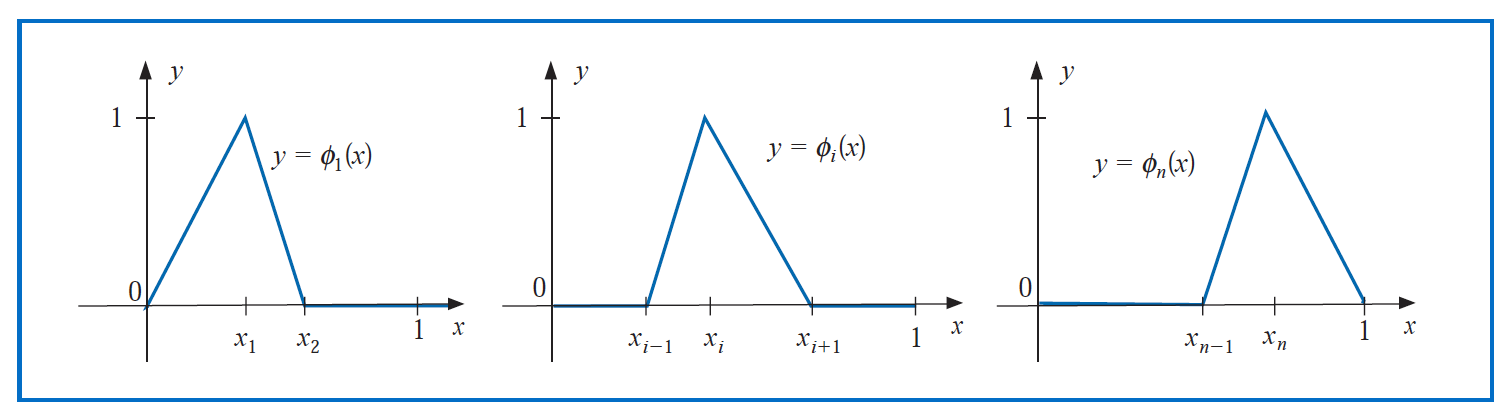
\includegraphics[width=1.0\linewidth]{splin.png}
\caption{\label{splin}Retirada de \cite{bur}}
\end{figure}
\begin{figure}[htb]
\centering
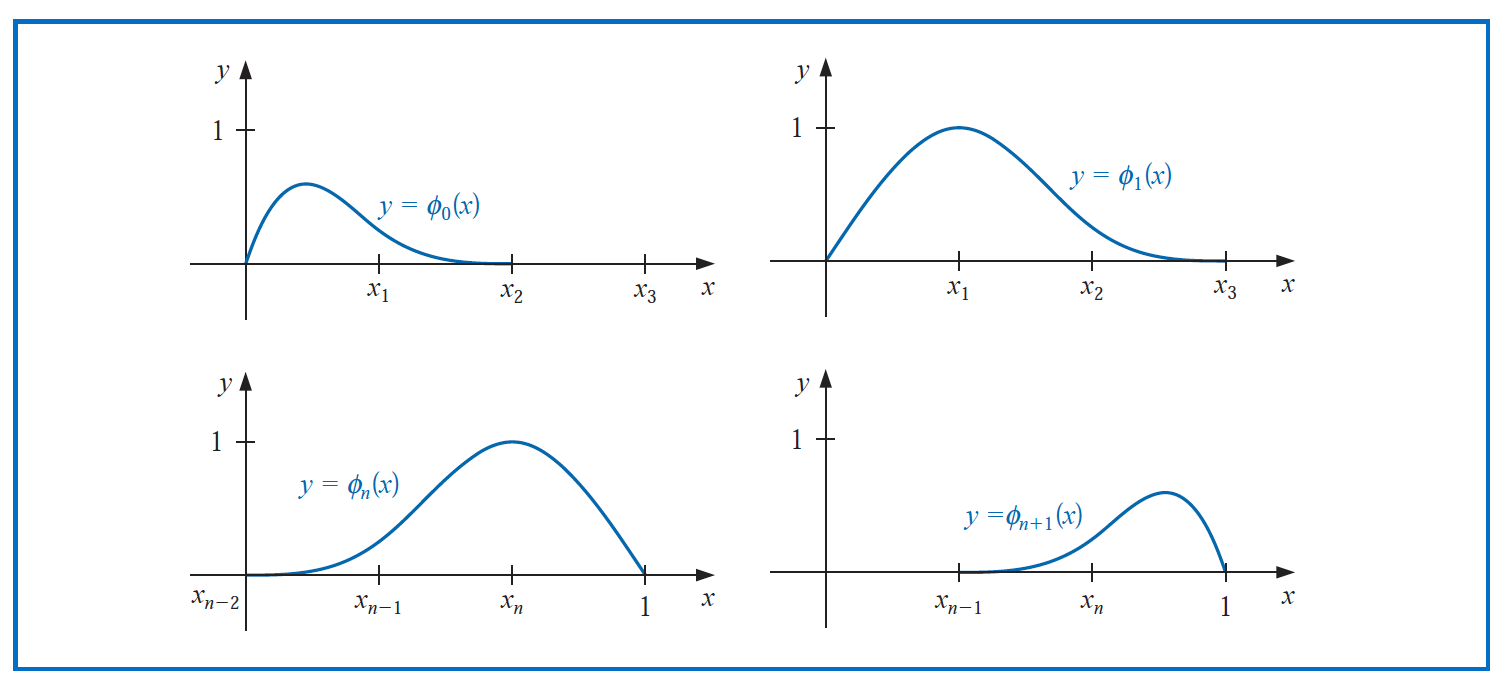
\includegraphics[width=1.0\linewidth]{spcub.png}
\caption{\label{spcub}Retirada de \cite{bur}}
\end{figure}\\
Para o caso em que $m=4$ (splines cúbicos), dados os elementos básicos $\phi_1,\phi_2,\dots,\phi_{n+4}$, descartam-se os primeiros três B-Splines e os três últimos B-Splines e, a partir deles são construídos 4 novos elementos básicos através das  combinações  $\phi_2(x) - 4\,\phi_1(x)$, $\phi_3(x)-\phi_1(x)$ e $\phi_{n-1}(x) - 4\,\phi_{n+4}(x)$, $\phi_{n-2}(x)-\phi_{n+4}(x)$	. Assim, obtêm-se novos elementos básicos $\phi_0,\phi_1,\dots,\phi_{n+1}$ conforme o mostra a Figura \ref{spcub}.\medskip\\
Tendo em mãos a base de splines, procede-se à montagem do sistema linear dado em \eqref{mmq}. Para tanto, foram necessárias algumas rotinas para a avaliação das integrais dadas pelos produtos internos $\langle \cdot,\cdot\rangle _L$ e $\langle \cdot,\cdot\rangle$. Essas e outra rotinas usadas no desenvolvimento deste trabalho são apresentadas na seguinte Seção.

\section*{Rotinas Utilizadas}
Nesta Seção são mostradas as rotinas (Subrotinas e Funções) usadas para a resolução do problema proposto. Todas elas foram implementadas na linguagem de programação Fortran 95 com compilador GFortran na versão 6.3.0.
\begin{itemize}
\item[•] \textbf{GaussBanda:} Esta função tem como objetivo resolver um sistema linear onde a matriz de coeficientes é uma matriz de banda. Os parâmetros de entrada são a matriz de banda, o vetor independente e o número de diagonais da matriz. Esta função retorna um vetor com a solução do sistema linear.

\item[•] \textbf{Horner:} O algoritmo de Horner é utilizado para a avaliação de polinômios e suas respectivas derivadas. Esta função recebe um polinômio em forma de vetor. Por exemplo, se o polinômio for $p(x)=a_0+a_1x+\cdots +a_nx^n$, então o vetor fornecido é  $[a_0\;\;a_1\;\cdots\; a_n]$. Também tem como parâmetro de entrada o ponto donde se deseja avaliar o polinômio (ou uma determinada derivada) e a ordem da derivada (se a ordem for 0 apenas se deseja conhecer o valor do polinômio no ponto dado). Esta função retorna o valor avaliado.

\item[•] \textbf{Fatorial:} Esta função, como seu nome o indica, calcula o fatorial de um número natural dado.

\item[•] \textbf{Norma:} Recebe como parâmetros de entrada dois vetores $u$ e $v$, e calcula a norma deles, dada por: $\|u-v\|=\dis\max_{1\leq i \leq n}|u(i)-v(i)|$, em que $n$ é a dimensão dos vetores $u$ e $v$.

\item[•] \textbf{ProdPoli:} Esta rotina recebe dois polinômios em forma de vetor (conforme foi indicado em Horner) e faz o produto deles.

\item[•] \textbf{SomPoli:} Como no caso anterior recebe dois polinômios e retorna a soma deles.

\item[•] \textbf{Translacao:} Esta função recebe como parâmetro de entrada um polinômio e um valor real $a$ e retorna o polinômio transladado $a$ unidades para a direita (caso $a>0$) ou $a$ unidades para a esquerda (caso $a<0$). Esta rotina desempenha uns dos papeis mais importante no desenvolvimento do projeto, pois uma vez construído o primeiro B-Spline, os demais elementos são obtidos por translação dele, devido a que o nós estão uniformemente espaçados.

\item[•] \textbf{BSplines:} Esta rotina constrói os polinômios definidos em \eqref{Qis}, ou seja, basicamente constrói a base de B-Splines. Recebe como parâmetros de entrada a ordem $m$ dos splines e o número de pontos interiores $n$ no intervalo $[0,1]$. Retorna um arranjo tridimensional contendo todos os polinômios $\mathcal{Q}_i^m$.

\item[•] \textbf{Particao:} O objetivo desta função é criar uma partição do intervalo $[0,1]$ e a partição estendida para a construção da base de B-Splines.

\item[•] \textbf{Romberg:} O Algoritmo de Romberg é utilizado para o calculo aproximado das integrais dadas pelos produtos internos definidos acima. Neste caso, é usado para o produto interno $\langle \cdot,\cdot\rangle _L$ definido no Método de Rayleigh-Ritz. Recebe como parâmetros de entrada dois B-Splines e os limites inferior e superior da integral definida. 

\item[•] \textbf{Rombergb:} Neste caso, o Algoritmo de Romberg é aplicado para calcular a integral dada pelo produto interno usual. Recebe um B-Spline e os correspondentes limites de integração.

\item[•] \textbf{ProdIntUsual:} Definição do produto interno usual das funções contínuas.

\item[•] \textbf{ProdIntL:} Definição do produto interno $\langle \cdot,\cdot\rangle _L$.
\end{itemize}

\section*{Resultados Numéricos}
\subsection*{Condições de fronteira homogêneas}
\subsubsection*{Teste 1} Para este experimento sejam $k(x)=1$, $q(x)=0$ e $f(x)=\pi^2(\sin \pi x - 9\sin 3\pi x )$. A solução exata para o problema \eqref{eqprob} é dada por $u(x)=\sin\pi x -\sin 3\pi x$. São considerados os valores $n=7,\, 15,\, 31$ e 63.

\begin{figure}[htb]
\centering
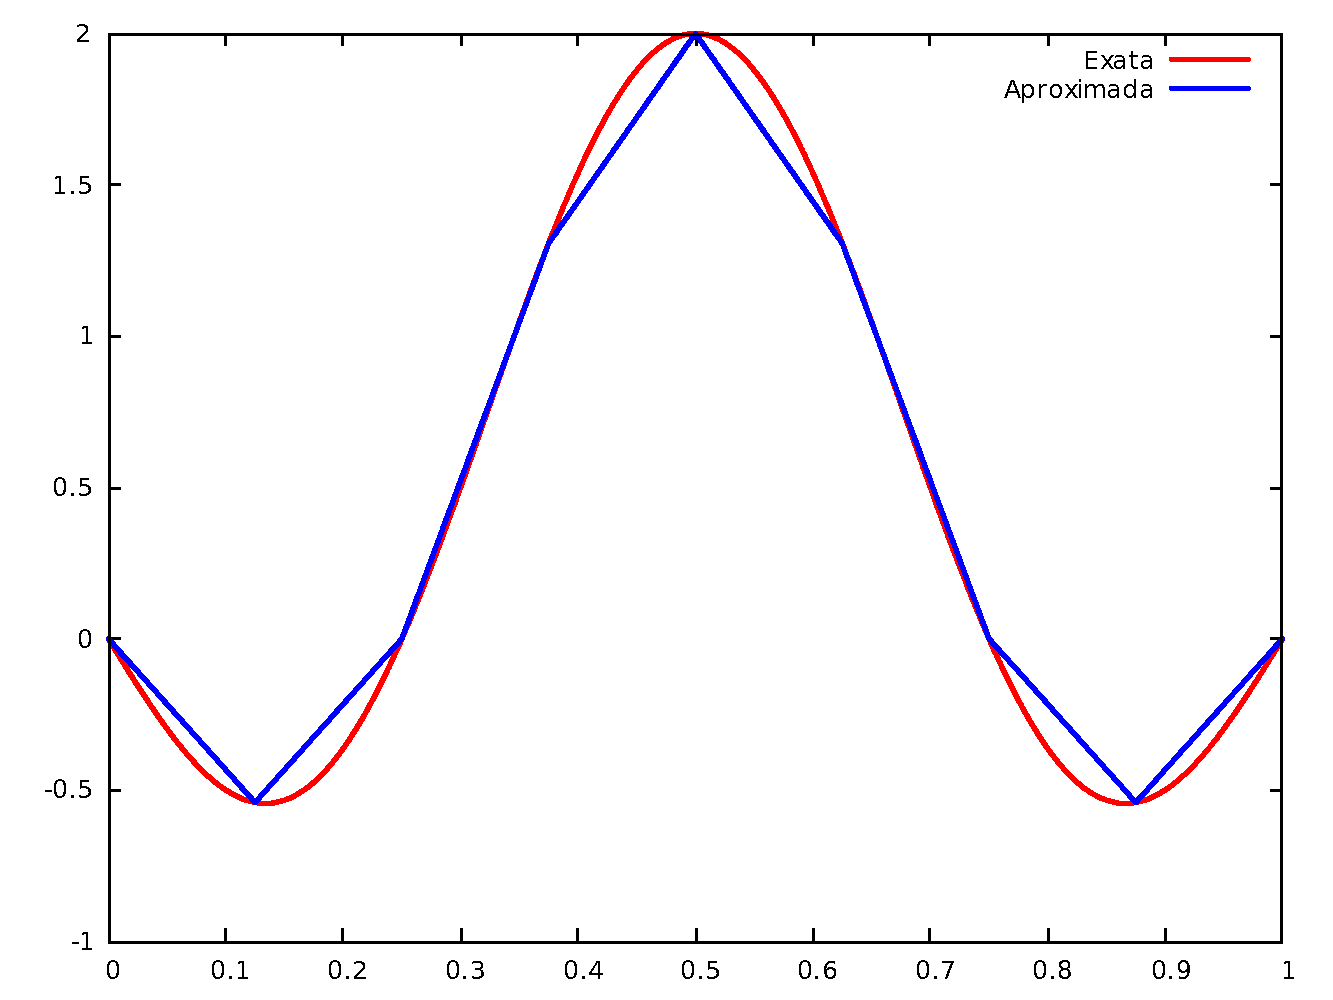
\includegraphics[width=0.8\linewidth]{splin7.pdf}
\caption{\label{splin}Resultado com Splines Lineares e $n=7$ para o Teste 1}
\end{figure}
\newpage
\begin{figure}[htb]
\centering
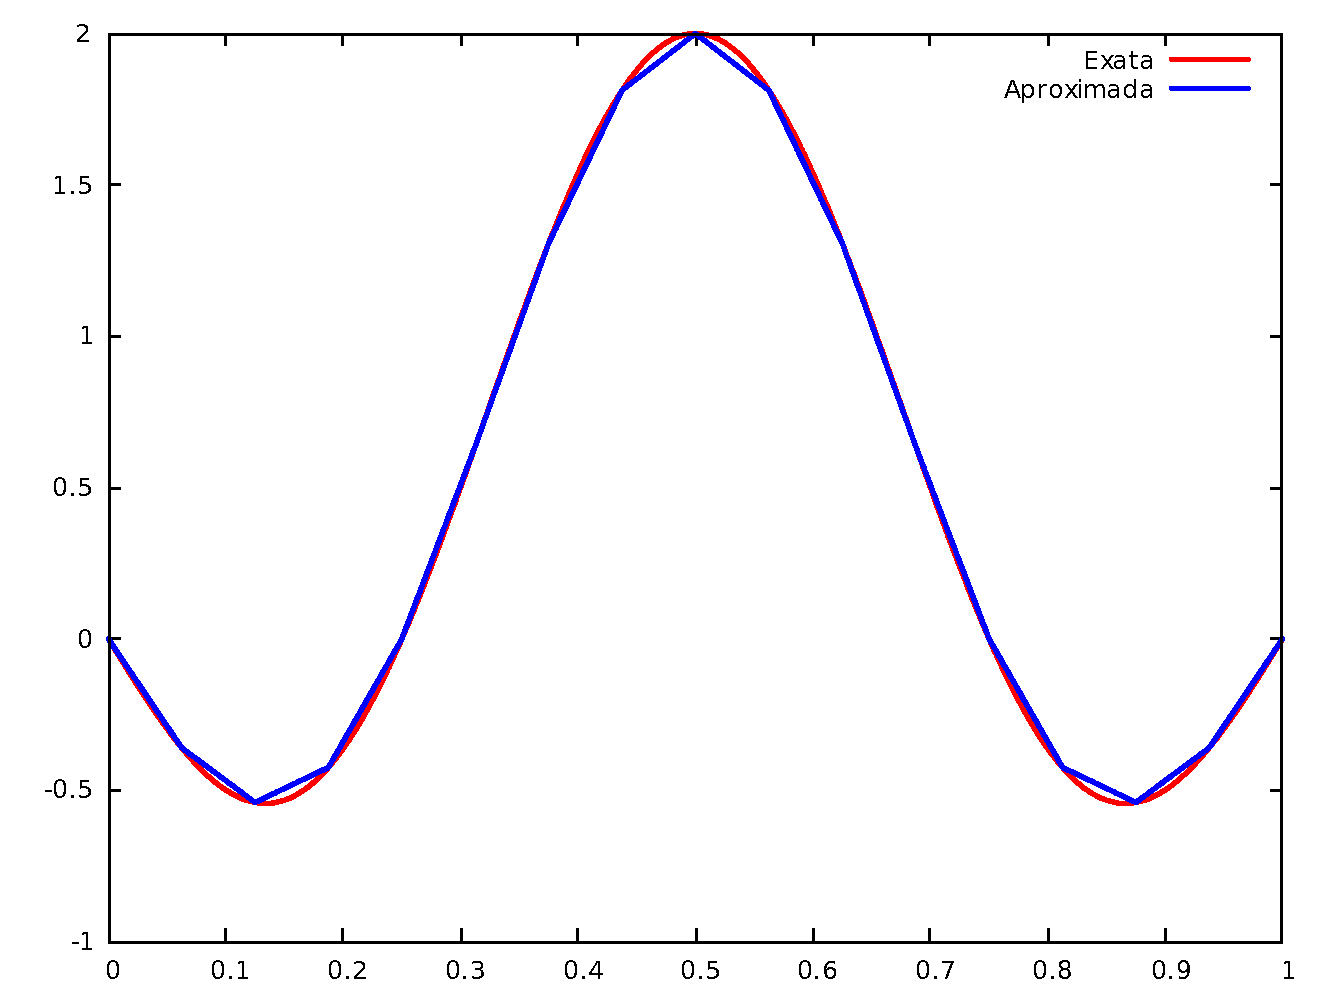
\includegraphics[width=0.8\linewidth]{splin15.pdf}
\caption{\label{splin}Resultado com Splines Lineares e $n=15$ para o Teste 1}
\end{figure}
\begin{figure}[h!]
\centering
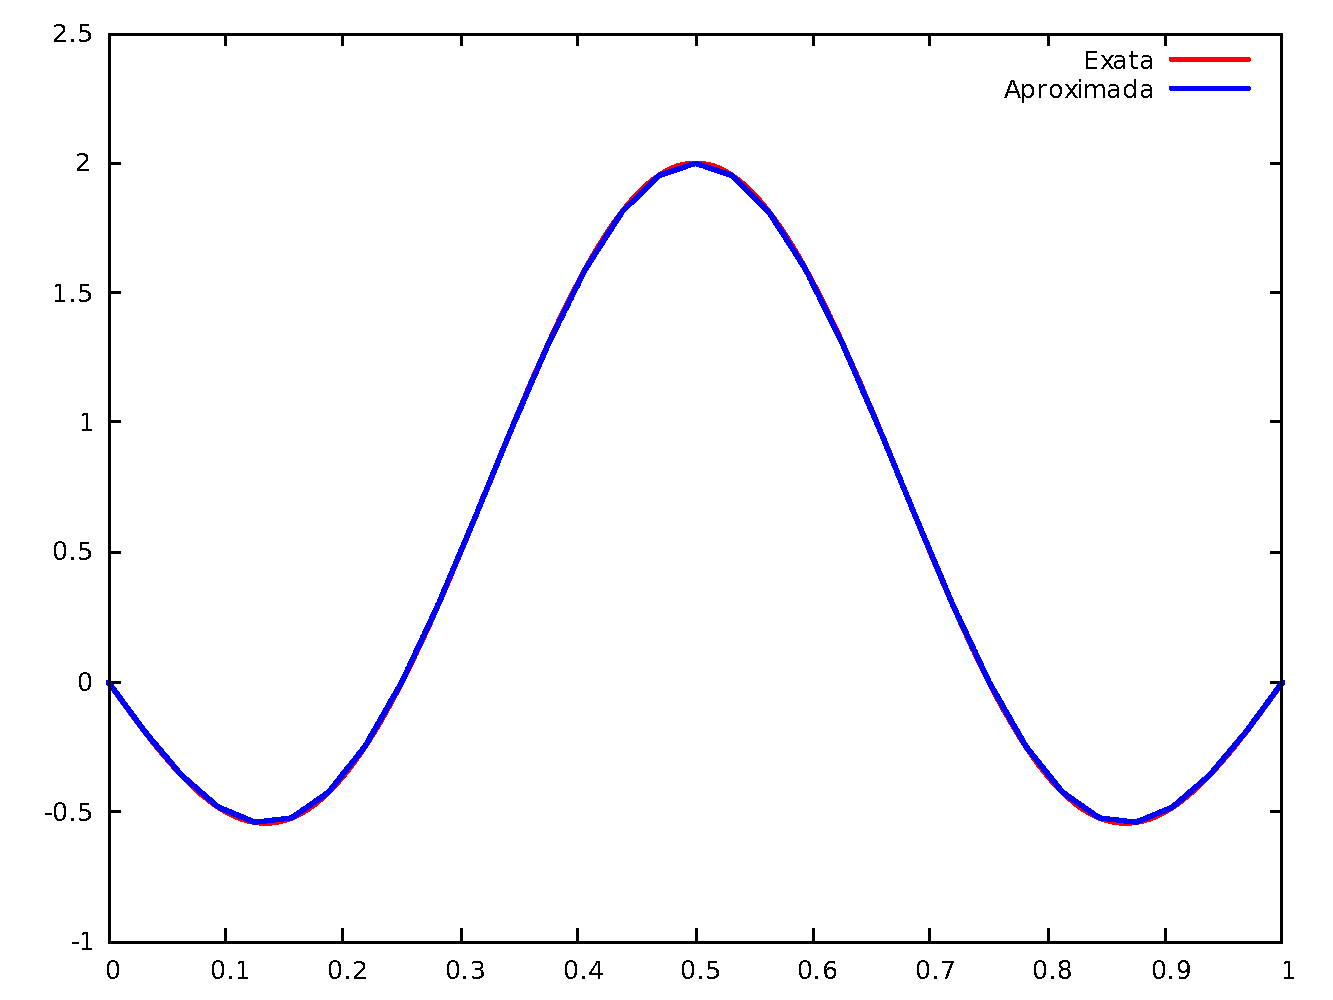
\includegraphics[width=0.8\linewidth]{splin31.pdf}
\caption{\label{splin}Resultado com Splines Lineares e $n=31$ para o Teste 1}
\end{figure}
\begin{figure}[h!]
\centering
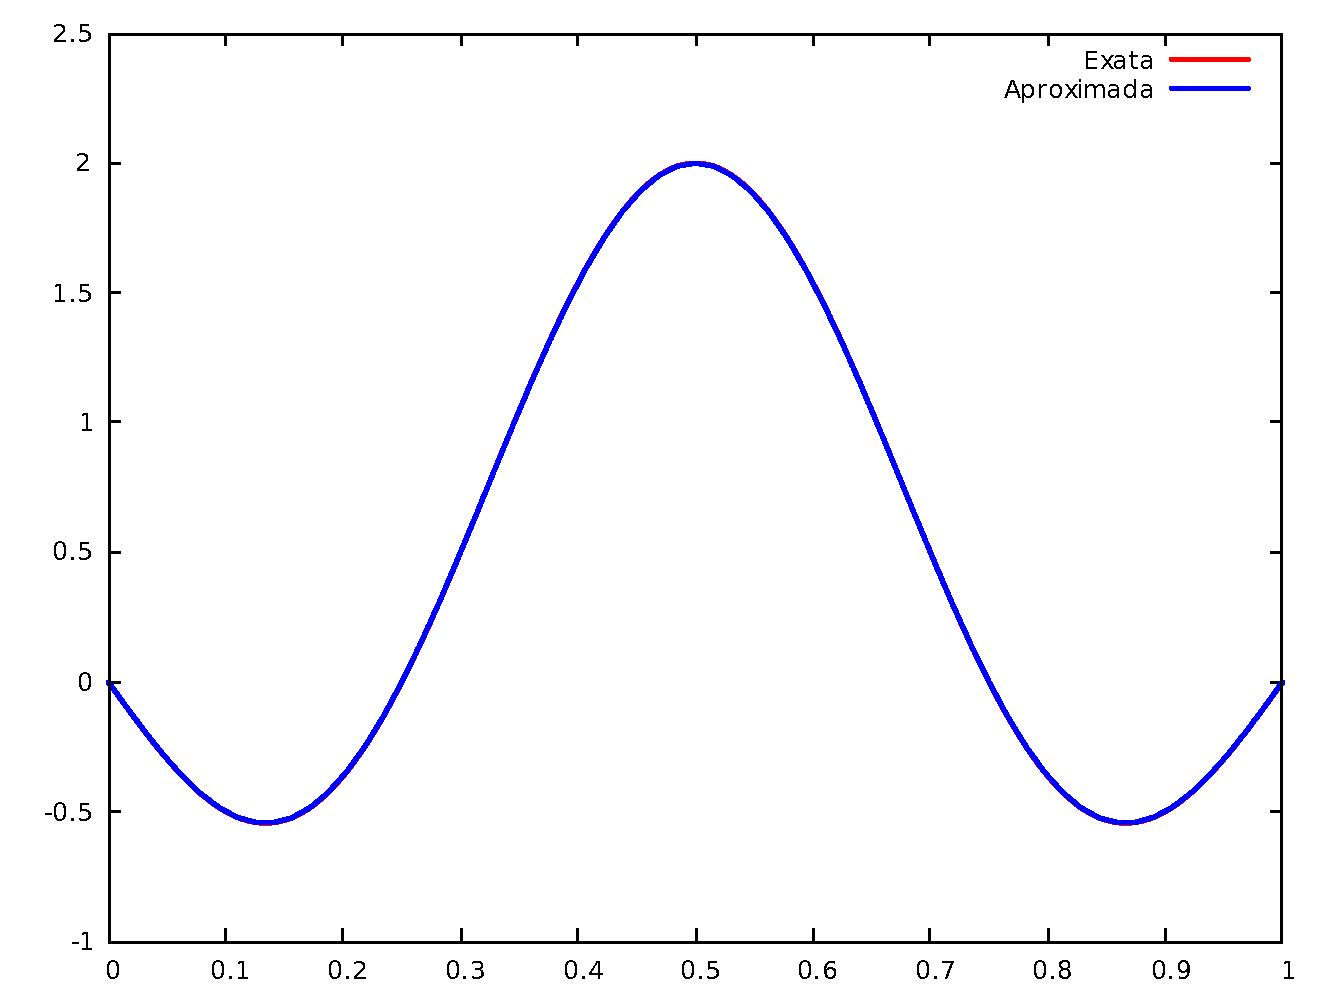
\includegraphics[width=0.8\linewidth]{splin63.pdf}
\caption{\label{splin}Resultado com Splines Lineares e $n=63$ para o Teste 1}
\end{figure}

\begin{figure}[H]
\centering
\subfigure[$n=7$]{
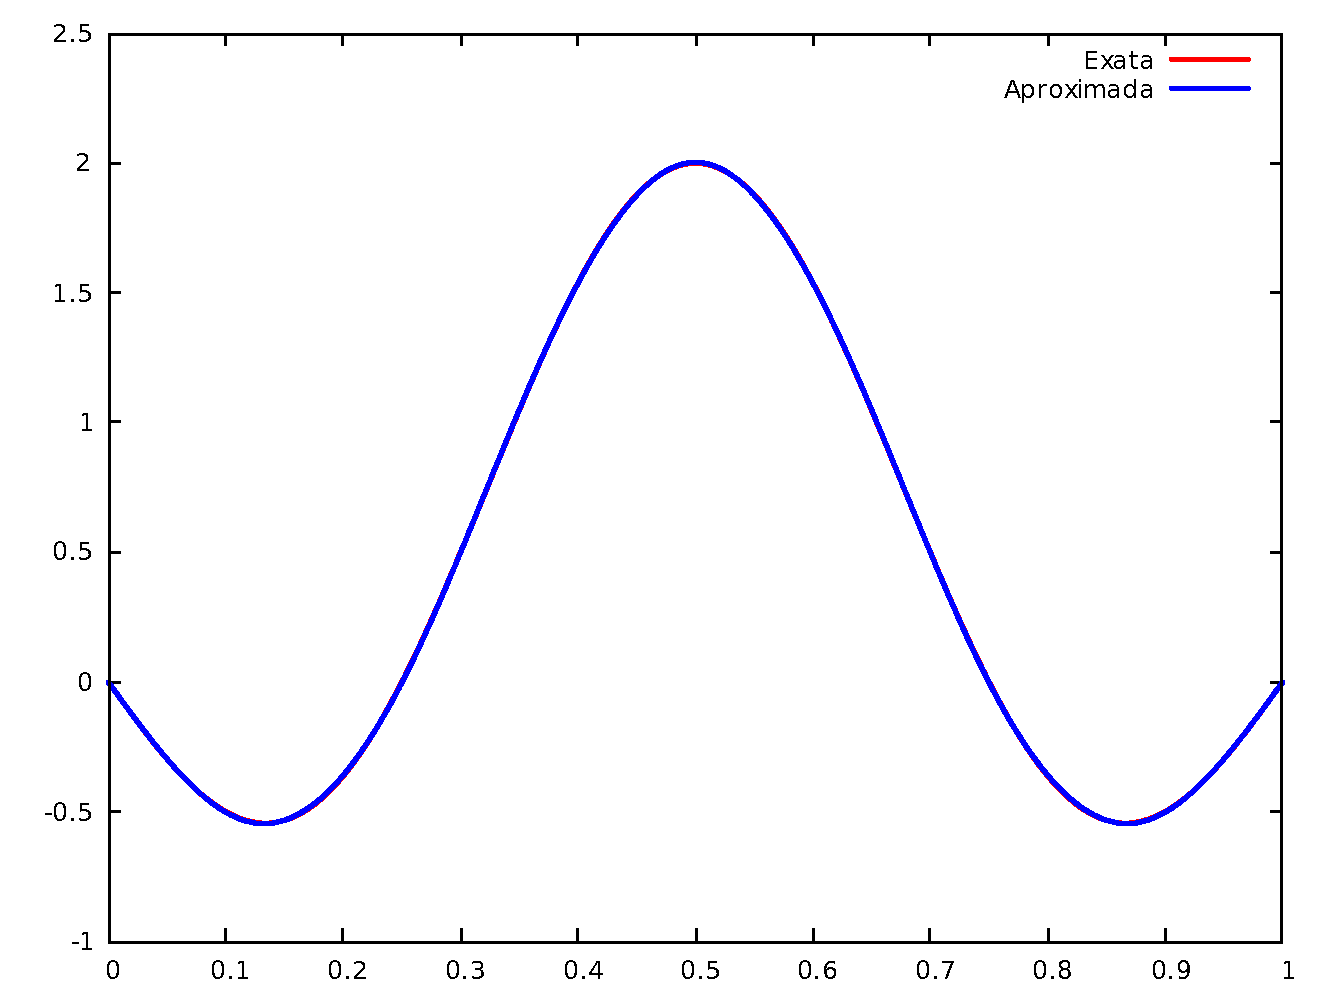
\includegraphics[width=0.48\linewidth]{spcub7.pdf}
}
\subfigure[$n=15$]{
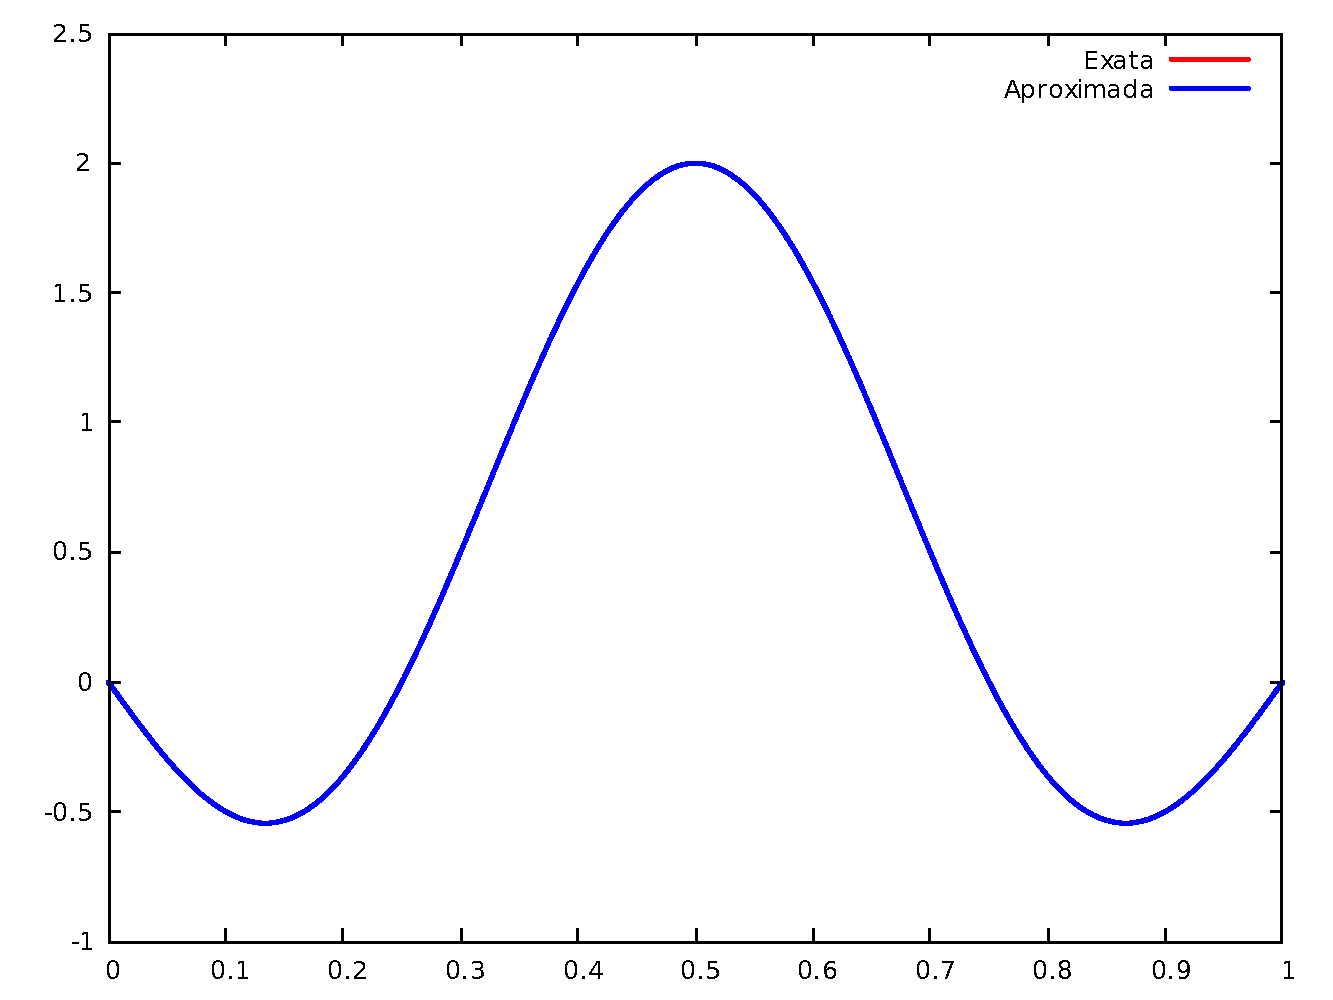
\includegraphics[width=0.48\linewidth]{spcub15.pdf}
}
\subfigure[$n=31$]{
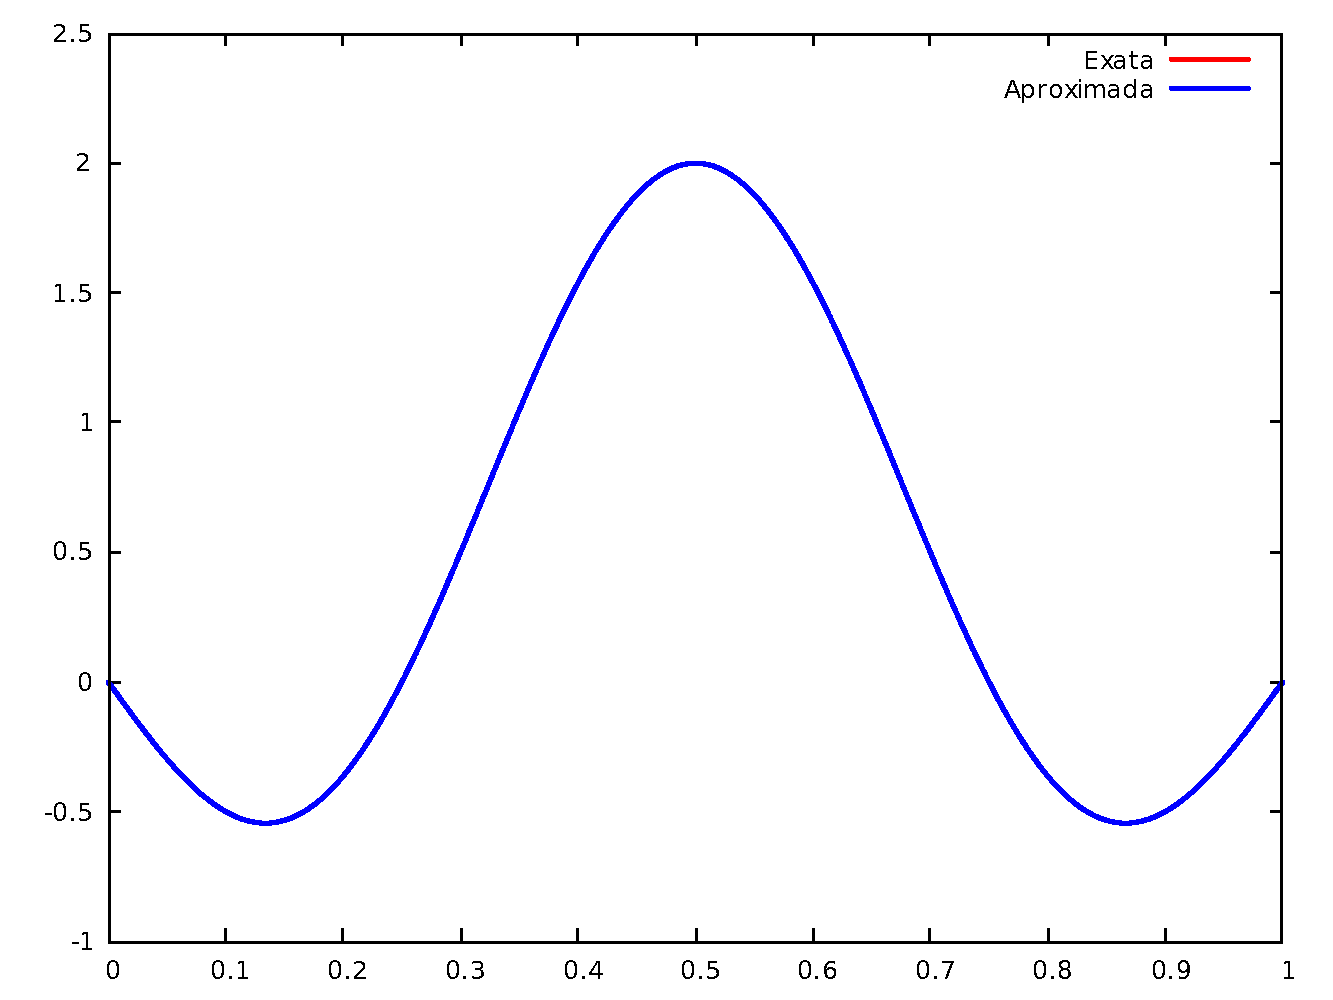
\includegraphics[width=0.48\linewidth]{spcub31.pdf}
}
\subfigure[$n=63$]{
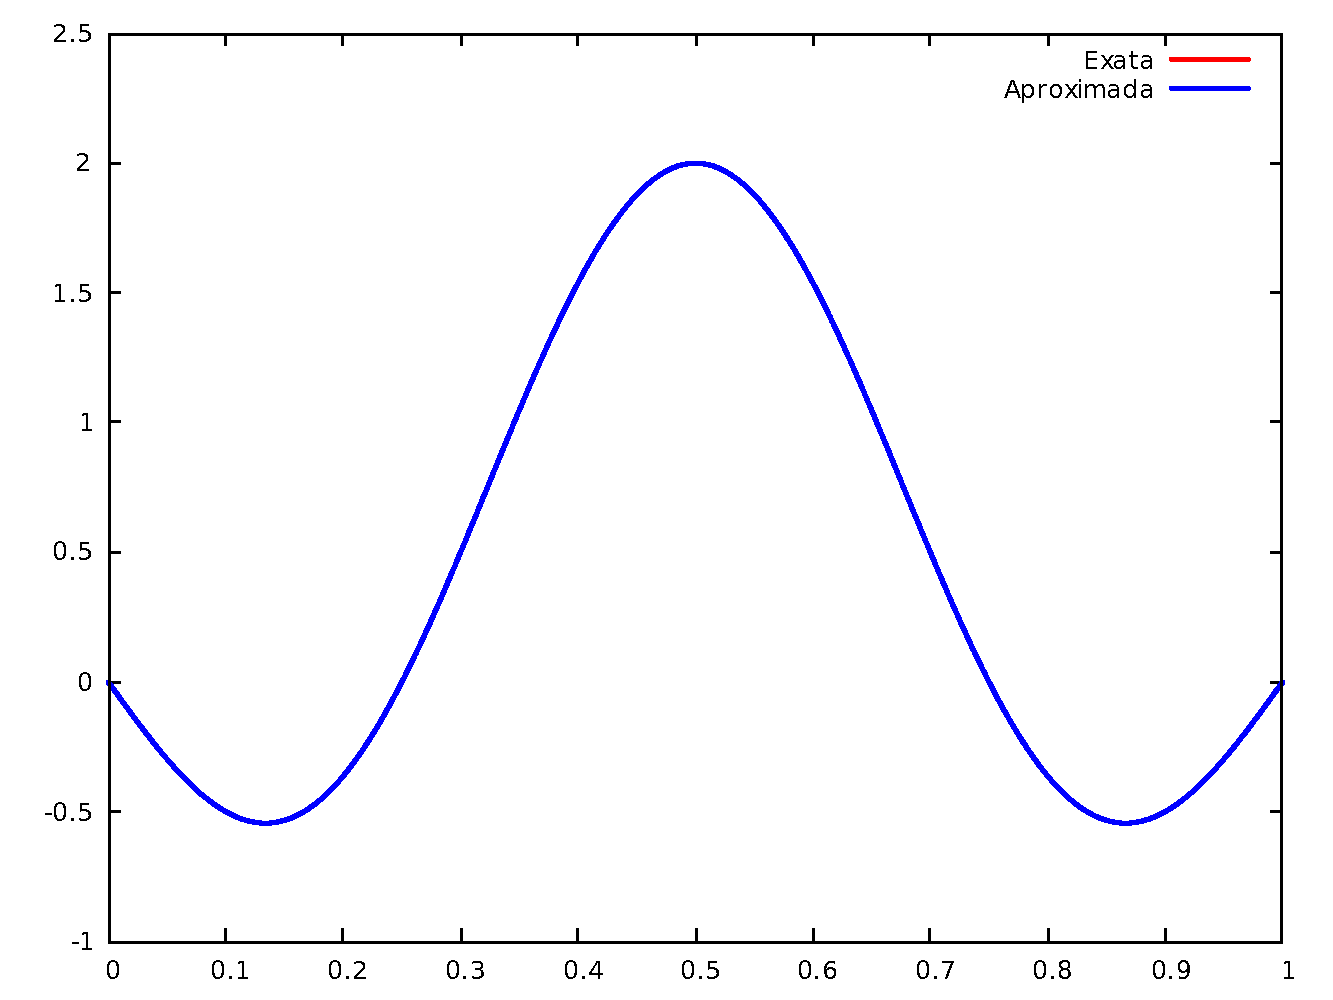
\includegraphics[width=0.48\linewidth]{spcub63.pdf}
}
\caption{Resultados com Splines Cúbicos para o Teste 1}
\end{figure}
\newpage
As Figuras 3, 4, 5 e 6 mostram os resultados para o caso de Splines Lineares. No caso dos Splines Cúbicos, note que já com $n=7$ tem-se uma boa aproximação com a solução exata conforme mostra a Figura 7. Na Tabela a seguir, mostra-se o erro e a ordem de convergência do método.
\begin{table}[h!]
\caption{\label{tabla4} Error e Ordem de convergência do Método com Splines Lineares e Splines Cúbicos para o Teste 1.}
\centering
  \begin{tabular}{l|cc|cc}
    \hline
    \hline
    \multirow{2}{*}{\textbf{$n$}} &
      \multicolumn{2}{c}{\textbf{Splines Lineares}} &\multicolumn{2}{c}{\textbf{Splines Cúbicos}} \\
    &\multicolumn{1}{c|}{Error} & \multicolumn{1}{c|}{Ordem} & \multicolumn{1}{c|}{Error} & \multicolumn{1}{c}{Ordem}\\
    \hline
    \hline
	7   & 0.159513968 & - & 4.08572184e-3  & - \\
	15 & 4.60059671e-2 & 3.4672 & 1.81805261e-4 & 22.473\\
	31 & 1.19095291e-2 & 3.8630 & 1.07697491e-5 & 16.881\\
	63 & 3.00329249e-3 & 3.9655 & 6.60525779e-7 & 16.305\\
    \hline
    \hline
  \end{tabular}
\end{table}

\subsubsection*{Teste 2} Para este teste, considera-se $k(x)=-1$, $q(x) = \dfrac{\pi^2}{4}$ e $f(x)=\dfrac{\pi^2}{16}\cos\dfrac{\pi}{4}x$. Neste caso, a solução exata do problema \eqref{eqprob} é dada por $u(x)=-\dfrac{1}{3}\cos\dfrac{\pi}{2}x - \dfrac{\sqrt{2}}{6}\sin\dfrac{\pi}{2}x + \dfrac{1}{3}\cos\dfrac{\pi}{4}x$. As Figuras abaixo mostram os resultados para $n=7$ e 15. Na Tabela 2, pode-se verificar que se satisfaz a ordem de convergência para os Splines Lineares e Cúbicos para $n=7,\, 15,\, 31$ e 63.	

\begin{figure}[htb]
\centering
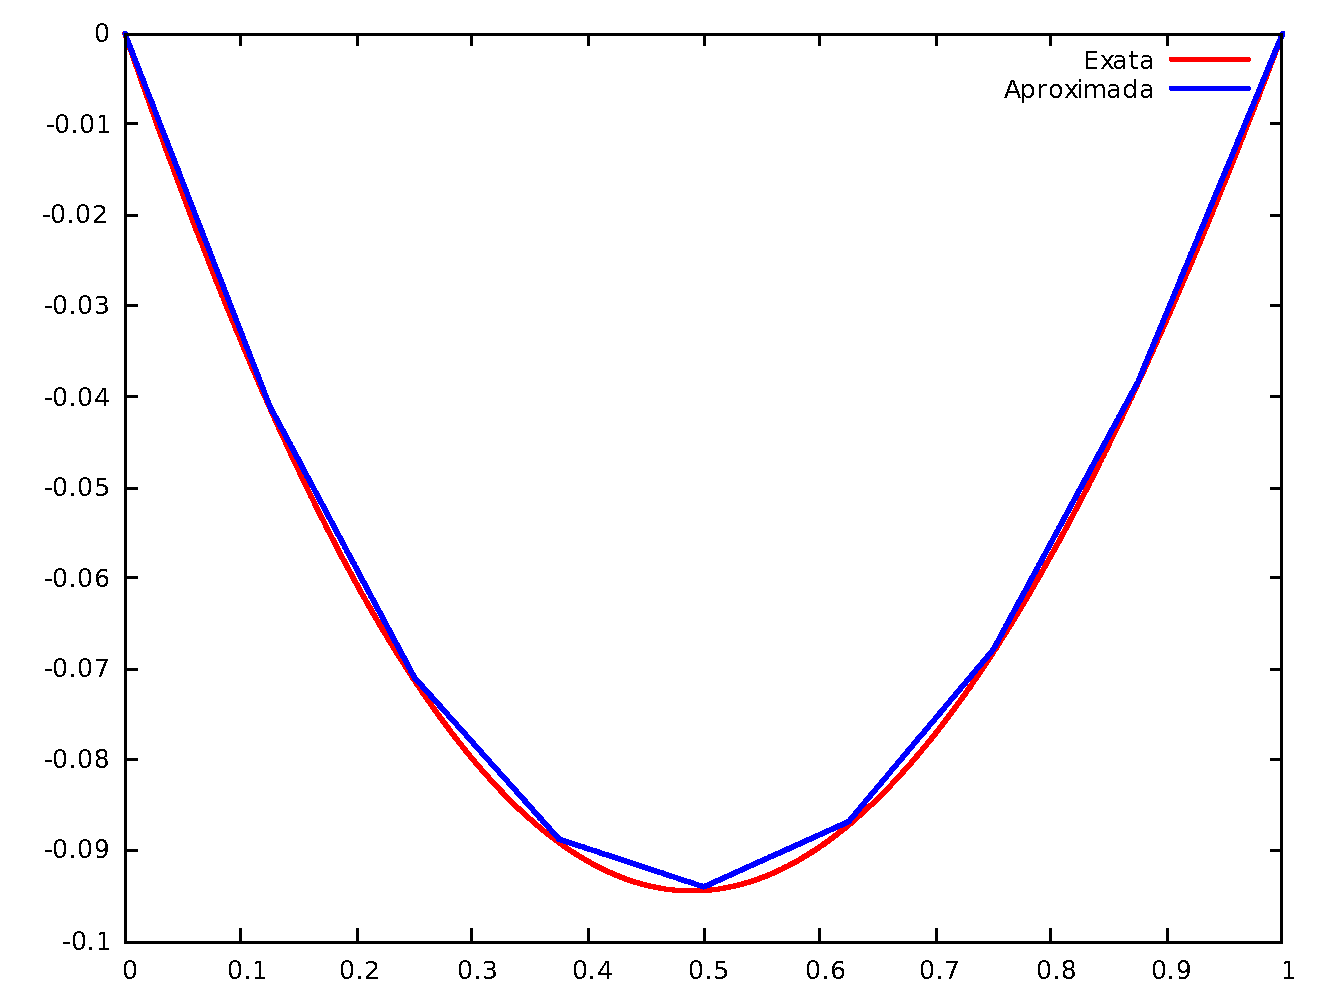
\includegraphics[width=0.8\linewidth]{t2splin7.pdf}
\caption{\label{splin}Resultado com Splines Lineares e $n=7$ para o Teste 2}
\end{figure}

\begin{figure}[t]
\centering
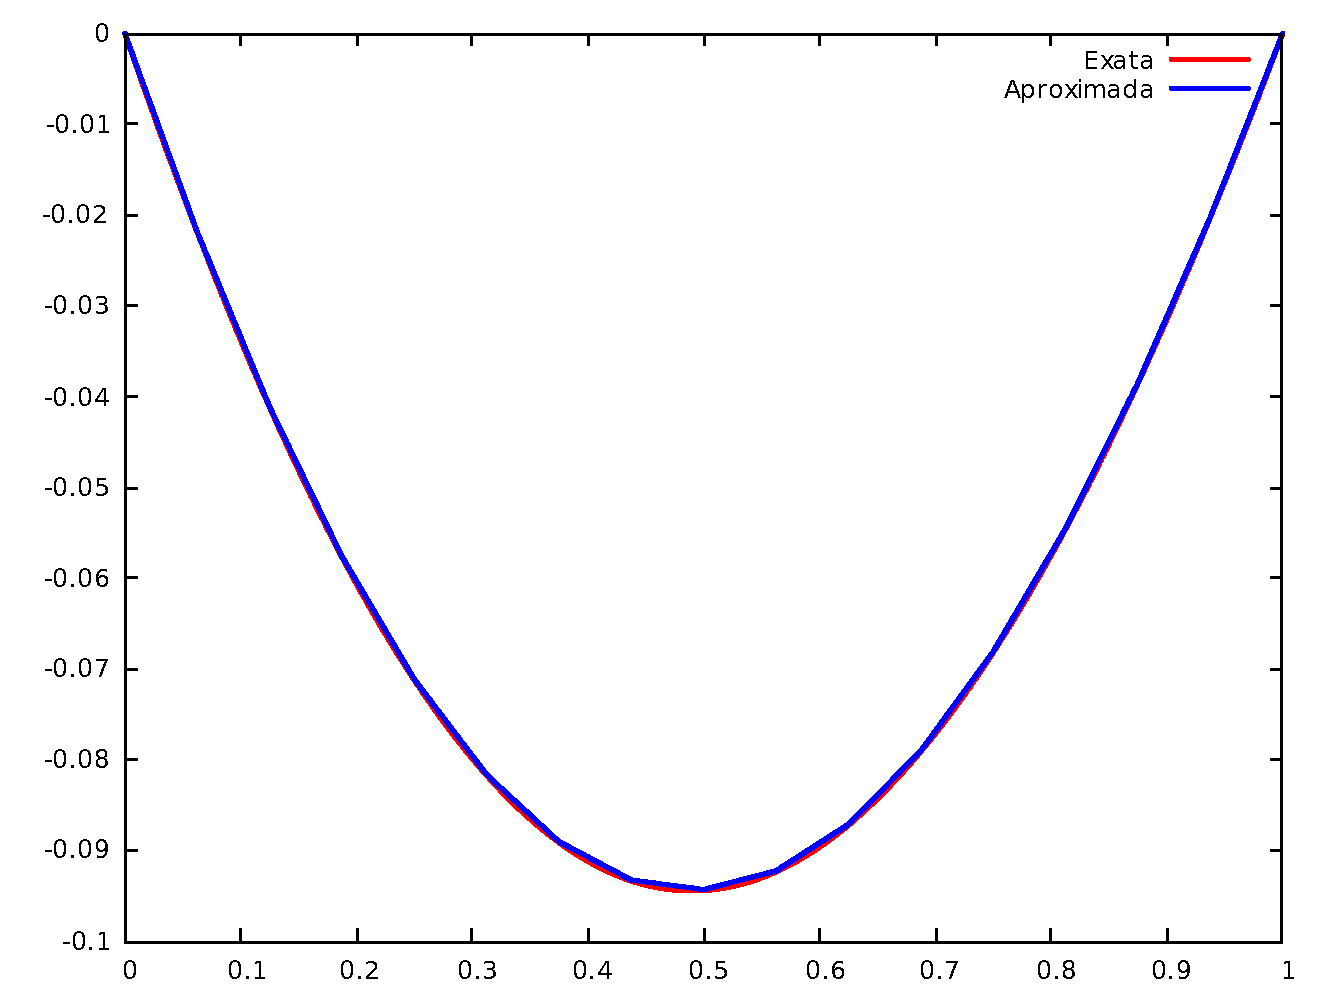
\includegraphics[width=0.8\linewidth]{t2splin15.pdf}
\caption{\label{splin}Resultado com Splines Lineares e $n=15$ para o Teste 2}
\end{figure}

\begin{figure}[H]
\centering
\subfigure[$n=7$]{
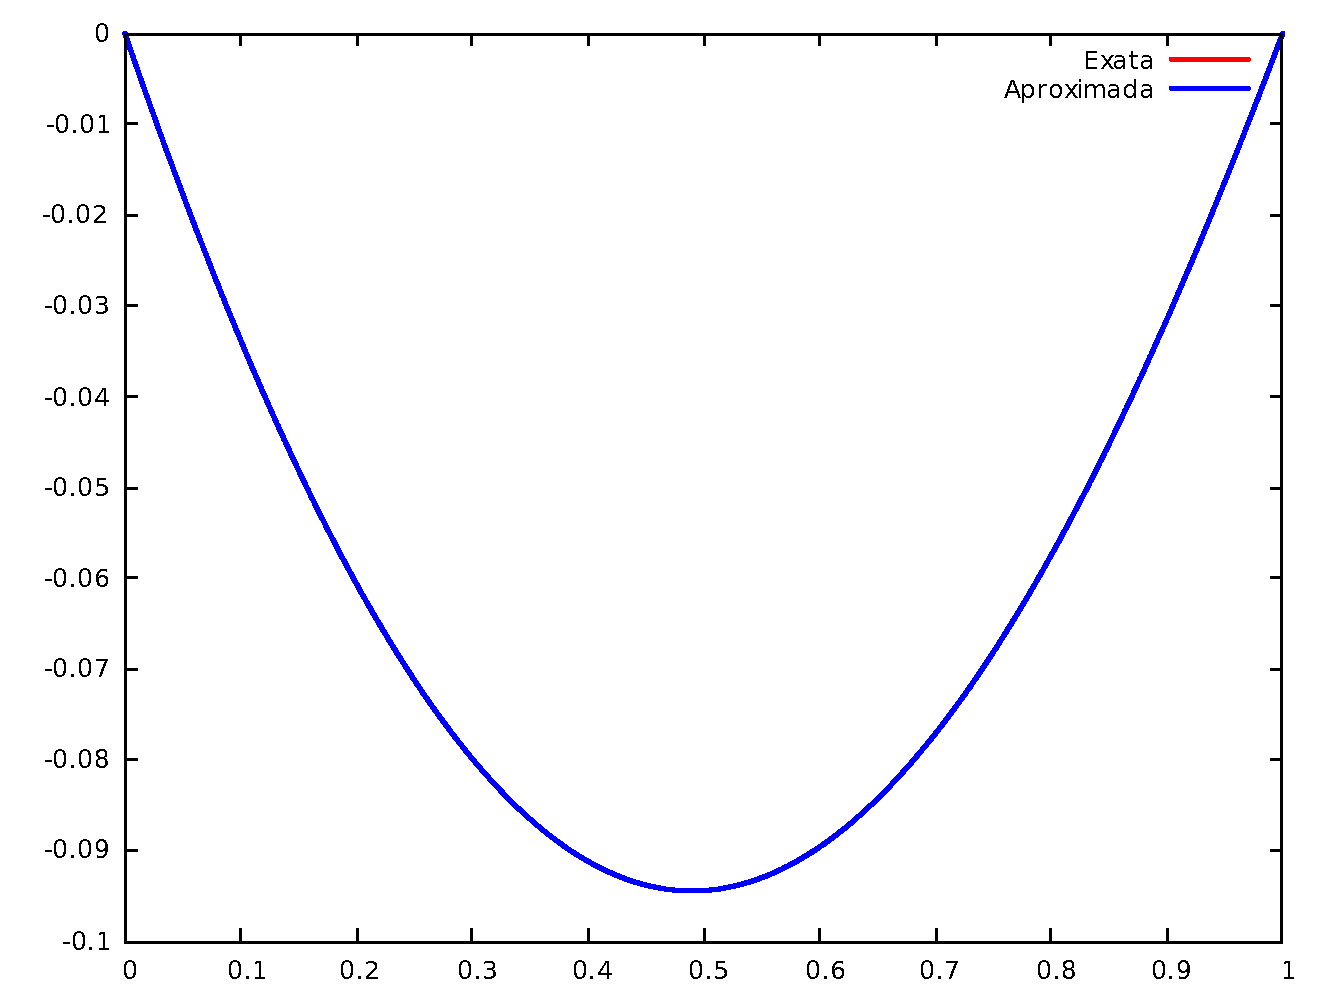
\includegraphics[width=0.48\linewidth]{t2spcub7.pdf}
}
\subfigure[$n=15$]{
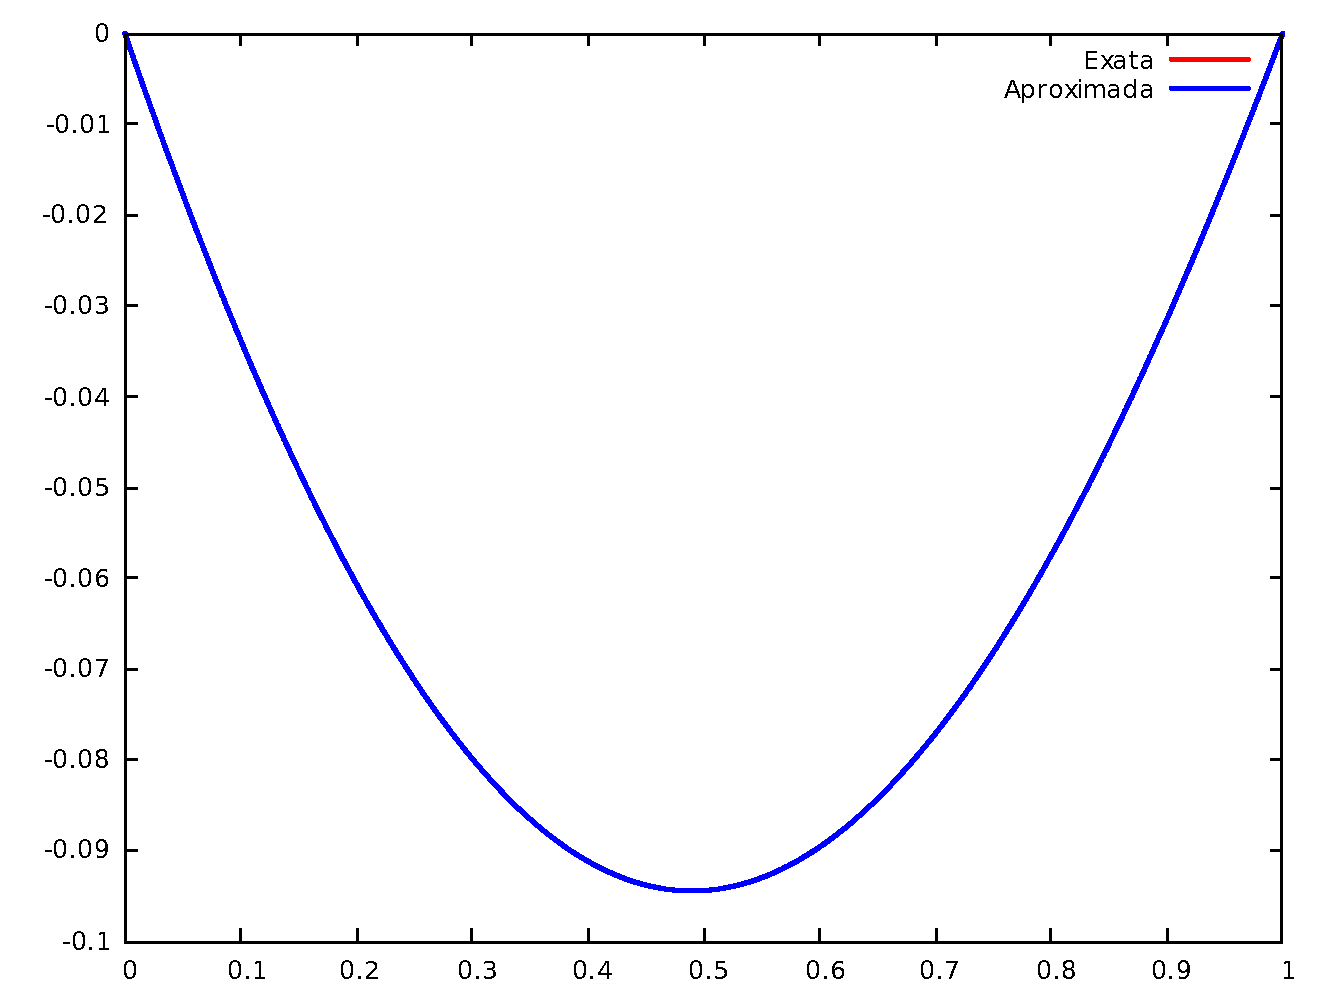
\includegraphics[width=0.48\linewidth]{t2spcub15.pdf}
}
\caption{Resultados com Splines Cúbicos para o Teste 2}
\end{figure}
\begin{table}[h!]
\caption{\label{tabla4} Error e Ordem de convergência do Método com Splines Lineares e Splines Cúbicos para o Teste 2.}
\centering
  \begin{tabular}{l|cc|cc}
    \hline
    \hline
    \multirow{2}{*}{\textbf{$n$}} &
      \multicolumn{2}{c}{\textbf{Splines Lineares}} &\multicolumn{2}{c}{\textbf{Splines Cúbicos}} \\
    &\multicolumn{1}{c|}{Error} & \multicolumn{1}{c|}{Ordem} & \multicolumn{1}{c|}{Error} & \multicolumn{1}{c}{Ordem}\\
    \hline
    \hline
	7   & 1.97446000e-3 & - & 8.36689157e-7  & - \\
	15 & 4.95315713e-4 & 3.9863 & 5.02801772e-8 & 16.641\\	
	31 & 1.24068432e-4 & 3.9923 & 3.13296430e-9 & 16.049\\
	63 & 3.10271653e-5 & 3,9987 & 1.95895286e-10 & 15.993\\
    \hline
    \hline
  \end{tabular}
\end{table}
\newpage
\subsection*{Condições de fronteira não homogêneas}
No caso de ter condições de fronteira não homogêneas, isto é, $u(0)=a$ e $u(1)=b$, em \eqref{eqprob}, pode-se reduzir este problema ao caso homogêneo resolvendo-se a equação
\begin{equation*}
L(v(x)) := f(x) + (b-a)k'(x)-q(x)(a+(b-a)x) = \hat{f}.
\end{equation*}
Vejamos que, neste caso, $u(x)=v(x)+a+(b-a)x$ é a solução da equação \eqref{eqprob} com condições de fronteira $u(0)=a$ e $u(1)=b$. Com efeito, note que $u'(x)=v'(x)+b-a$ e $u''(x)=v''(x)$. Então, $f(x) + (b-a)k'(x)-q(x)(a+(b-a)x)=$
\begin{eqnarray*}
 &=&(-k(x)\,u'(x))' + q(x)\,u(x) + (b-a)k'(x)- q(x)(a+(b-a)x)\\
&=& -k'(x)\,u'(x)-k(x)\,u''(x)+q(x)\,u(x) + (b-a)k'(x) - a\,q(x) - (b-a)x\,q(x)\\
&=& -k'(x)(v'(x)+b-a)-k(x)\,v''(x) + q(x)(v(x)+a+(b-a)x) + (b-a)k'(x)-a\,q(x)-\\
&-& (b-a)x\,q(x)	\\
&=& -k'(x)v'(x)-k(x)v''(x)+q(x)v(x)\\
&=& \hat{f}.
\end{eqnarray*}
Portanto, $u$ é solução do problema \eqref{eqprob} com condições de fronteira $u(x)=v(x)+a+(b-a)x$.

\subsubsection*{Teste 3} Neste experimento considera-se as mesmas funções do Teste 1, com condições de fronteira $u(0)=1$ e $u(1)=2$. Note que o erro e a Ordem de convergência do Método são iguais aos obtidos nos Teste 1, conforme o mostra a Tabela 3.

\begin{figure}[H]
\centering
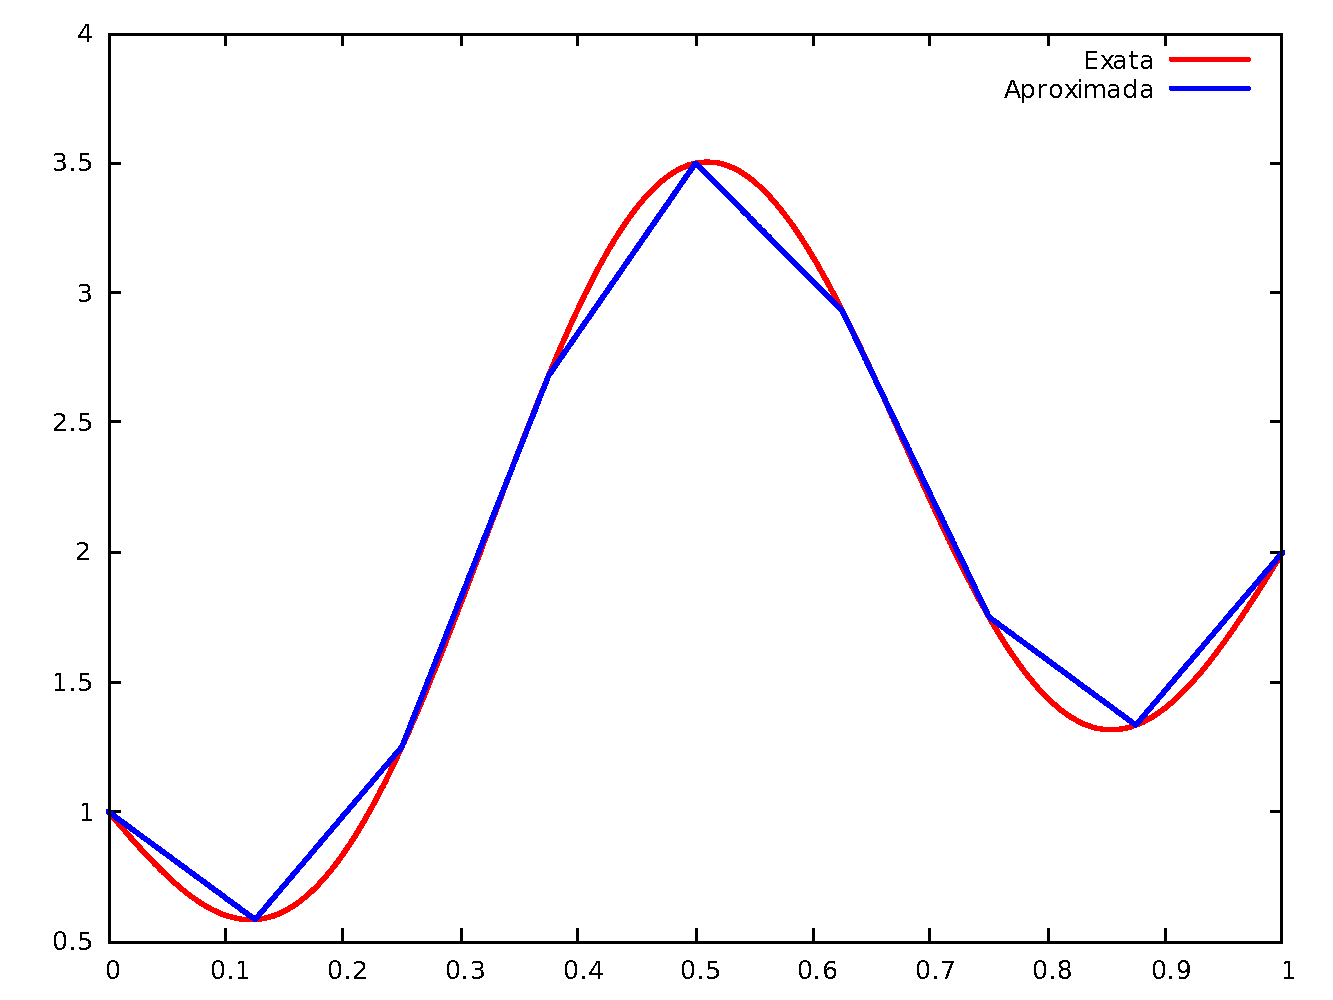
\includegraphics[width=0.8\linewidth]{t3splin7.pdf}
\caption{\label{splin}Resultado com Splines Lineares e $n=7$ para o Teste 3}
\end{figure}
\begin{figure}[H]
\centering
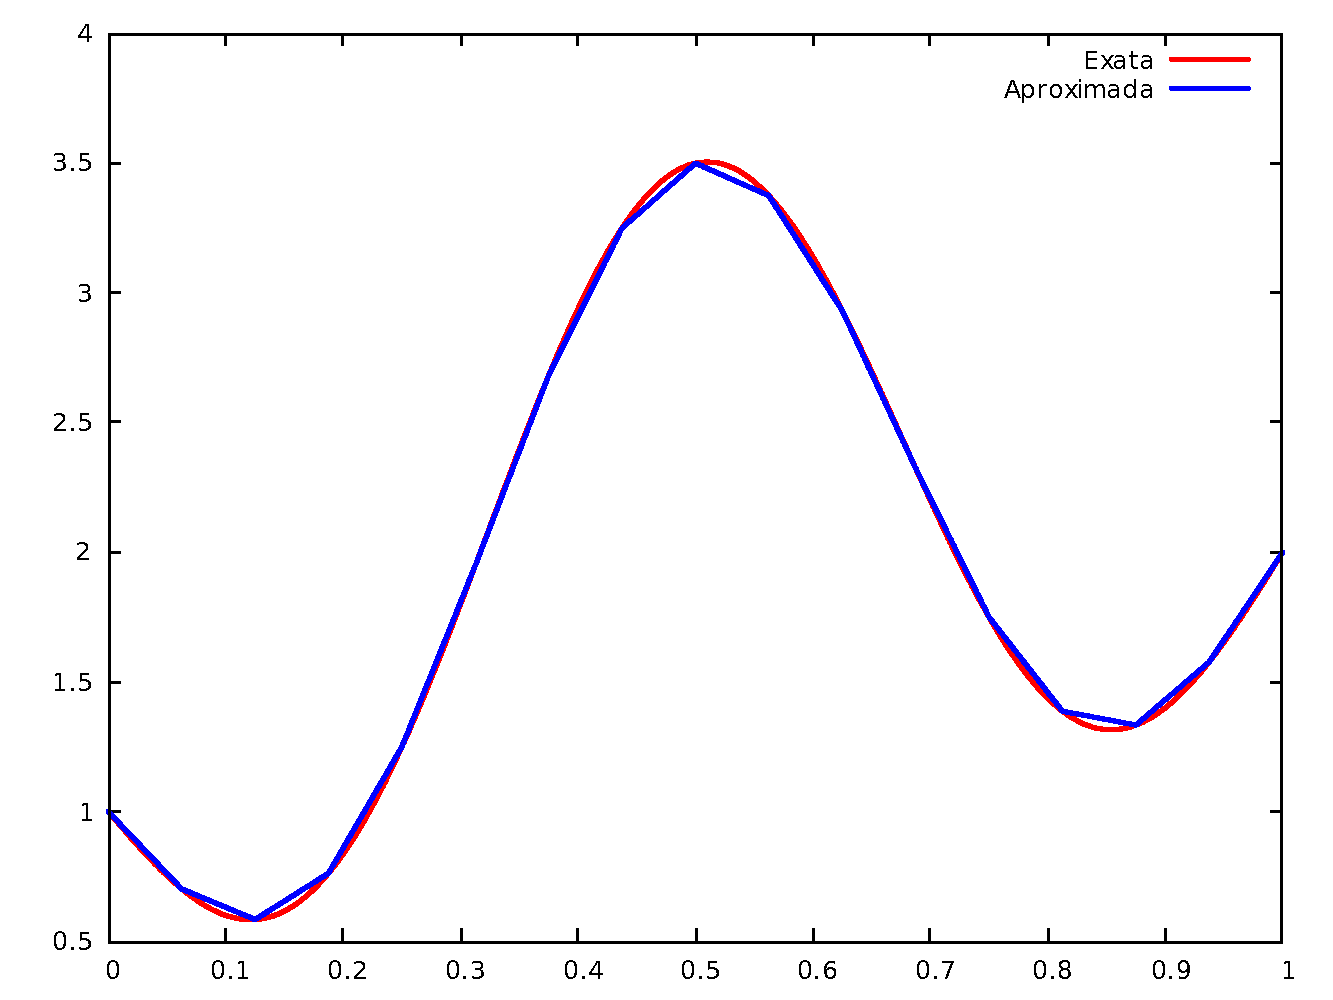
\includegraphics[width=0.8\linewidth]{t3splin15.pdf}
\caption{\label{splin}Resultado com Splines Lineares e $n=15$ para o Teste 3}
\end{figure}
\begin{figure}[H]
\centering
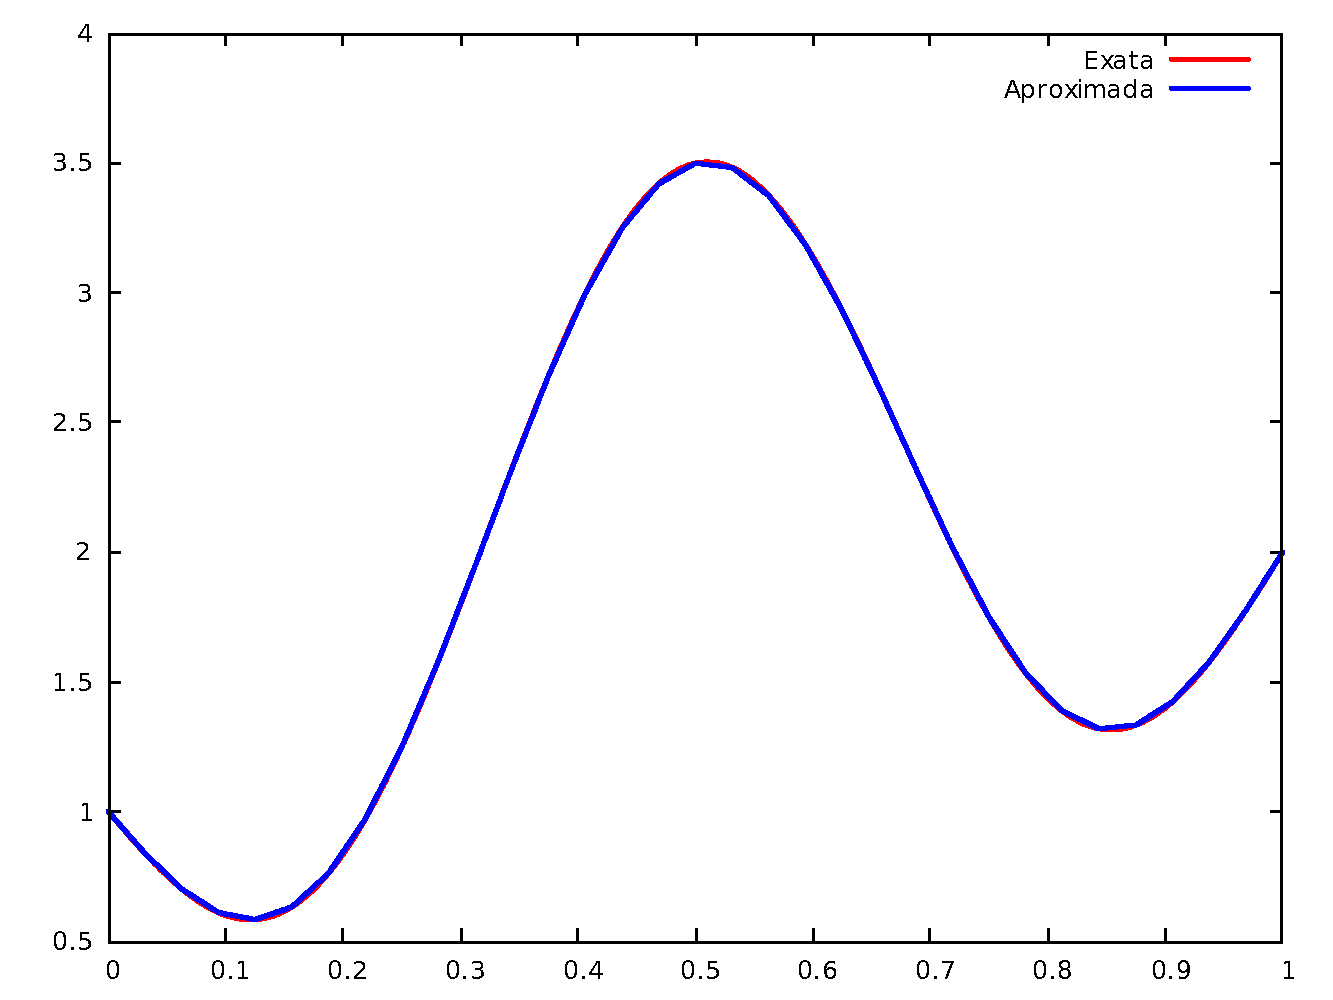
\includegraphics[width=0.8\linewidth]{t3splin31.pdf}
\caption{\label{splin}Resultado com Splines Lineares e $n=31$ para o Teste 3}
\end{figure}
\begin{figure}[H]
\centering
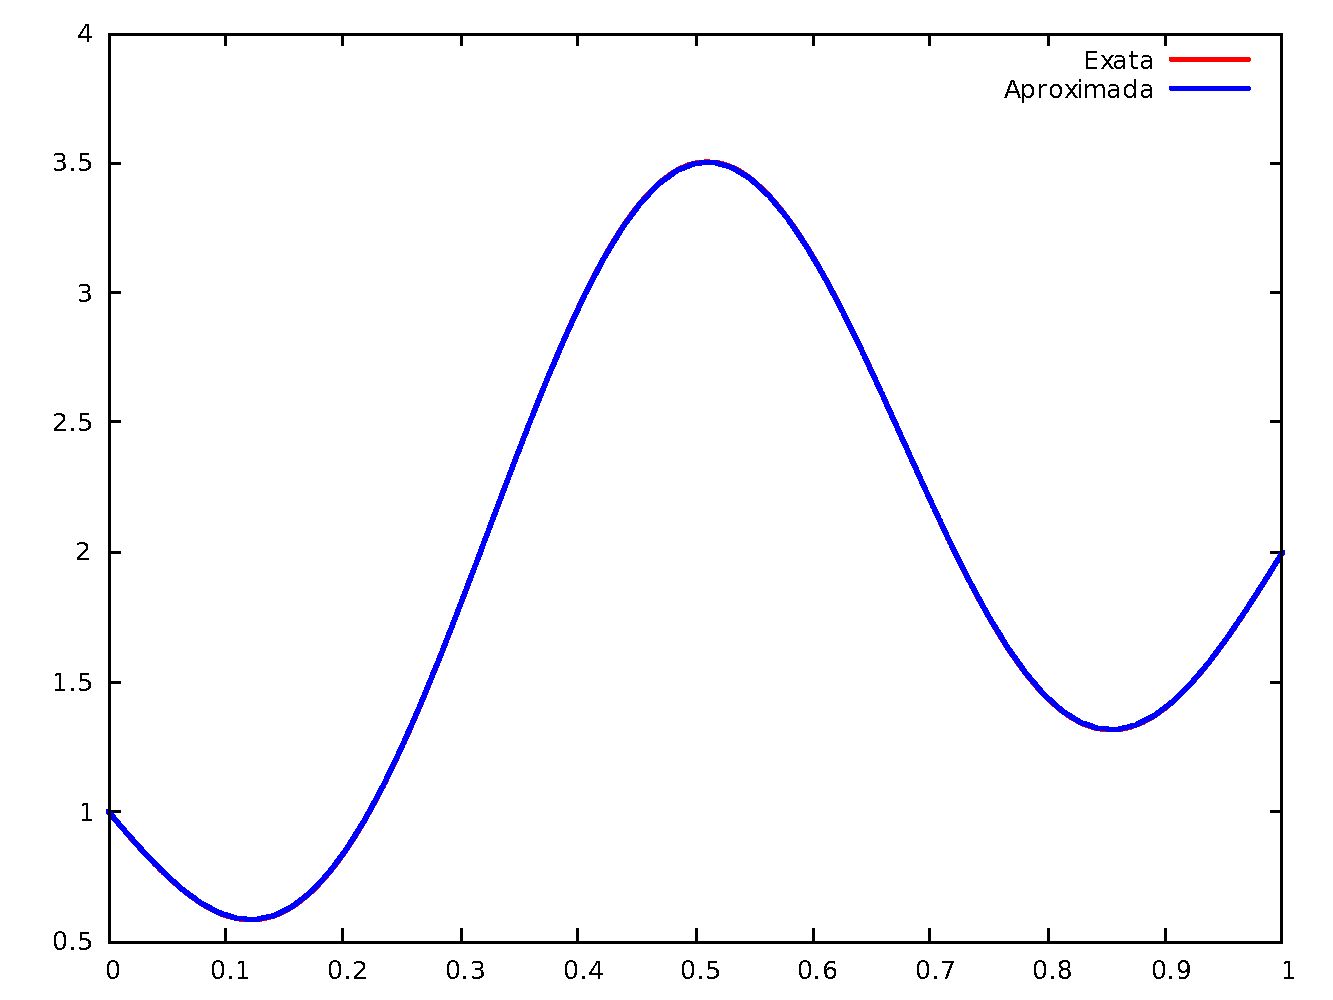
\includegraphics[width=0.7\linewidth]{t3splin63.pdf}
\caption{\label{splin}Resultado com Splines Lineares e $n=63$ para o Teste 3}
\end{figure}

\begin{figure}[H]
\centering
\subfigure[$n=7$]{
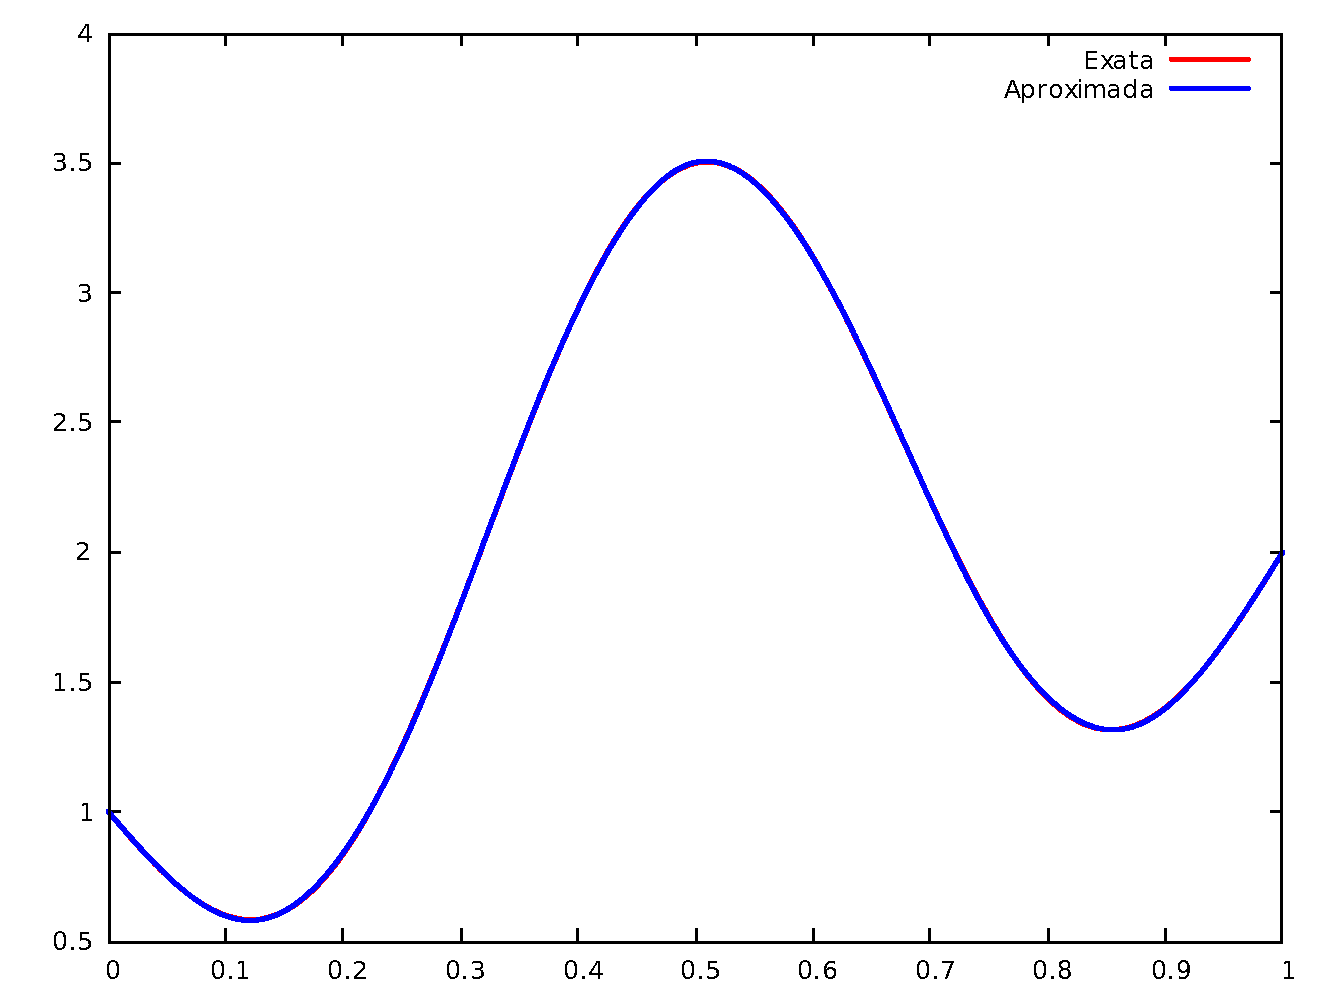
\includegraphics[width=0.48\linewidth]{t3spcub7.pdf}
}
\subfigure[$n=15$]{
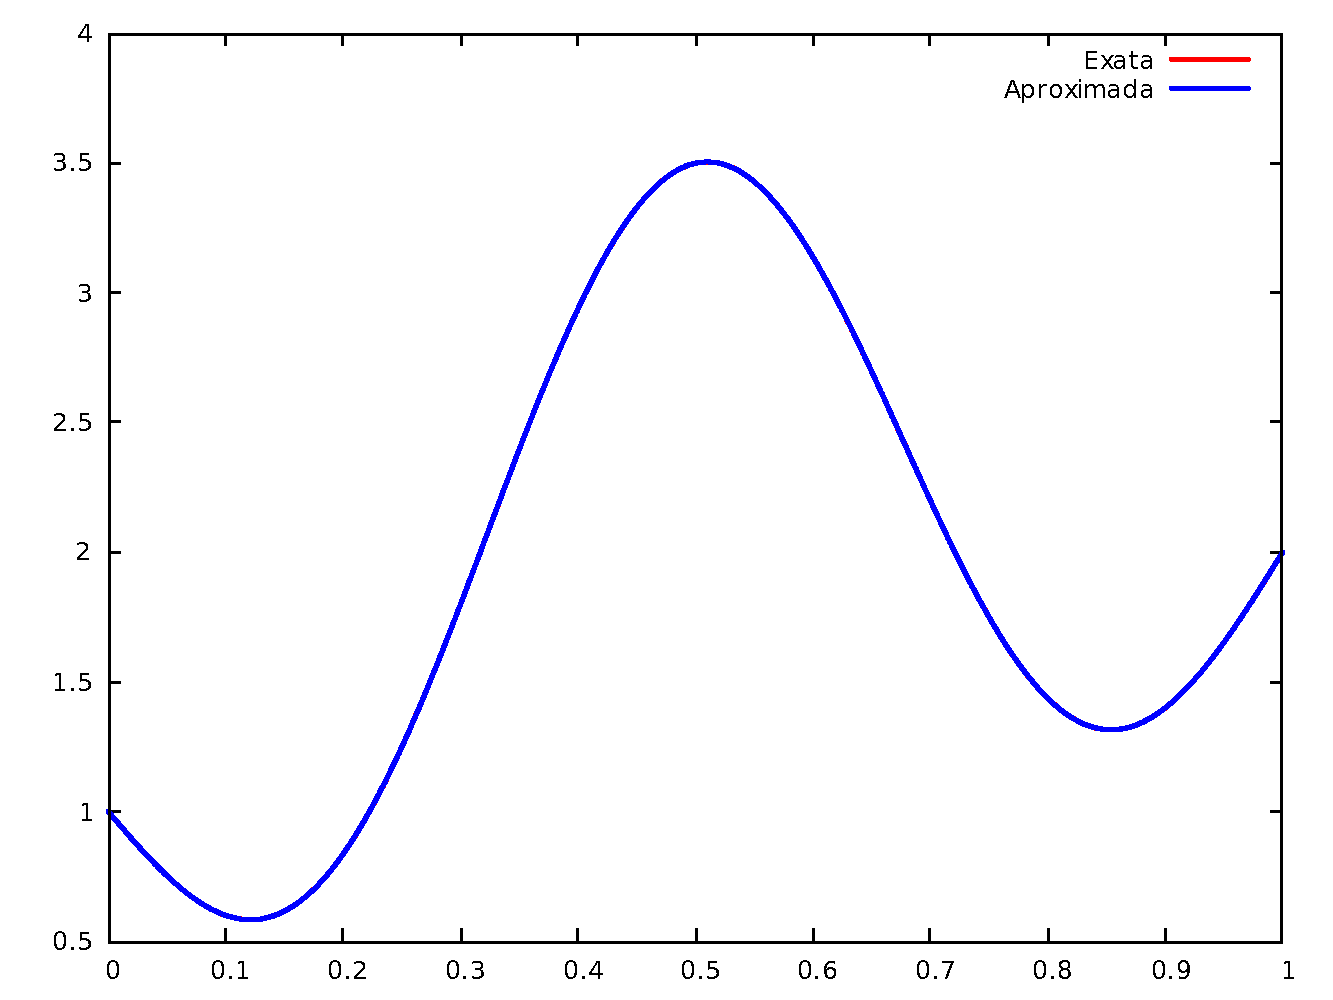
\includegraphics[width=0.48\linewidth]{t3spcub15.pdf}
}
\subfigure[$n=31$]{
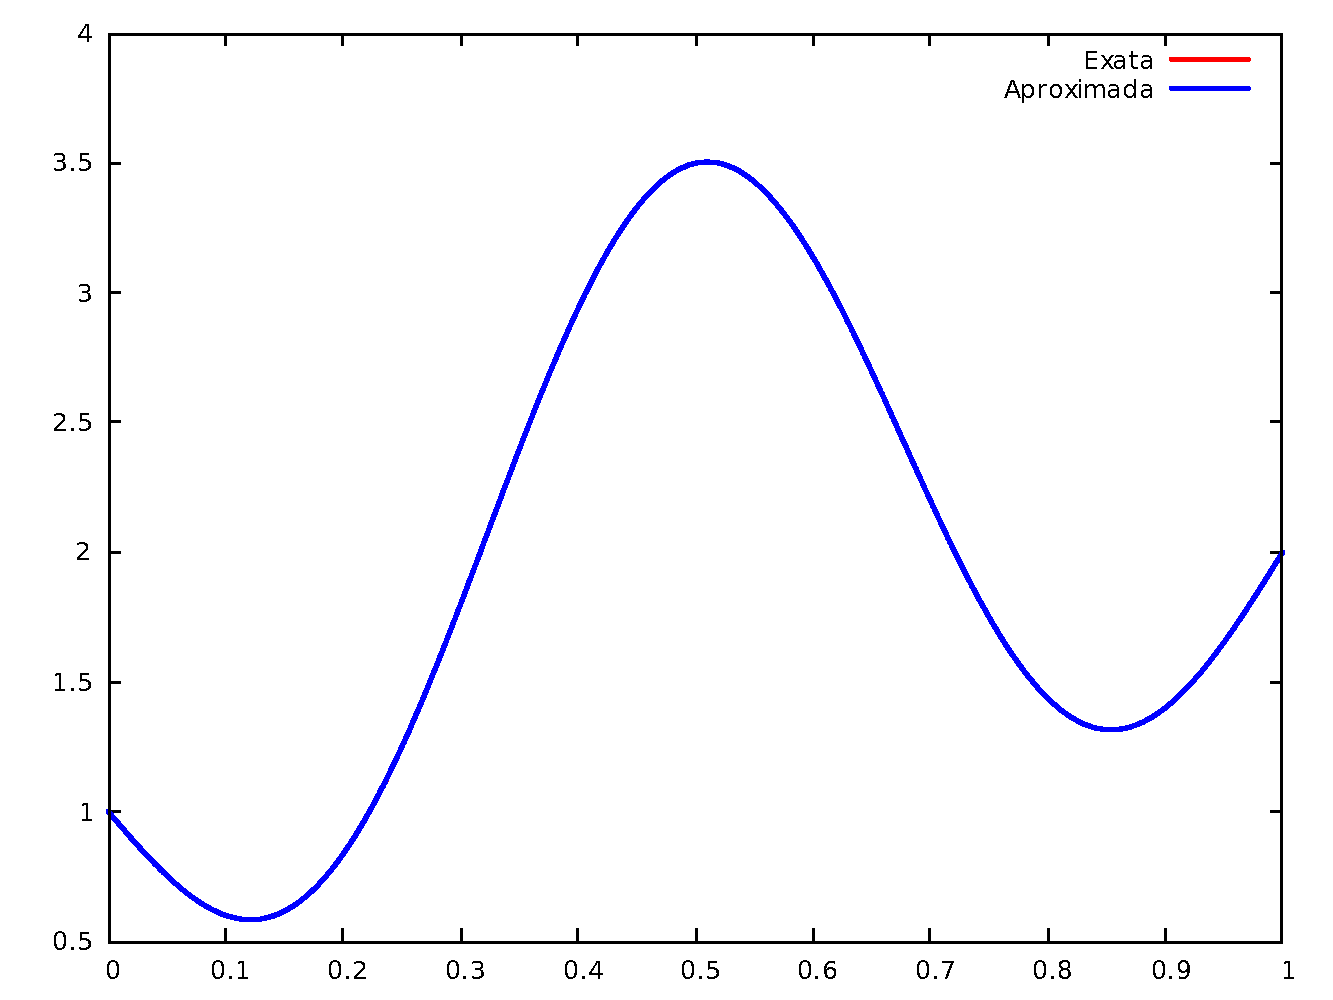
\includegraphics[width=0.48\linewidth]{t3spcub31.pdf}
}
\subfigure[$n=63$]{
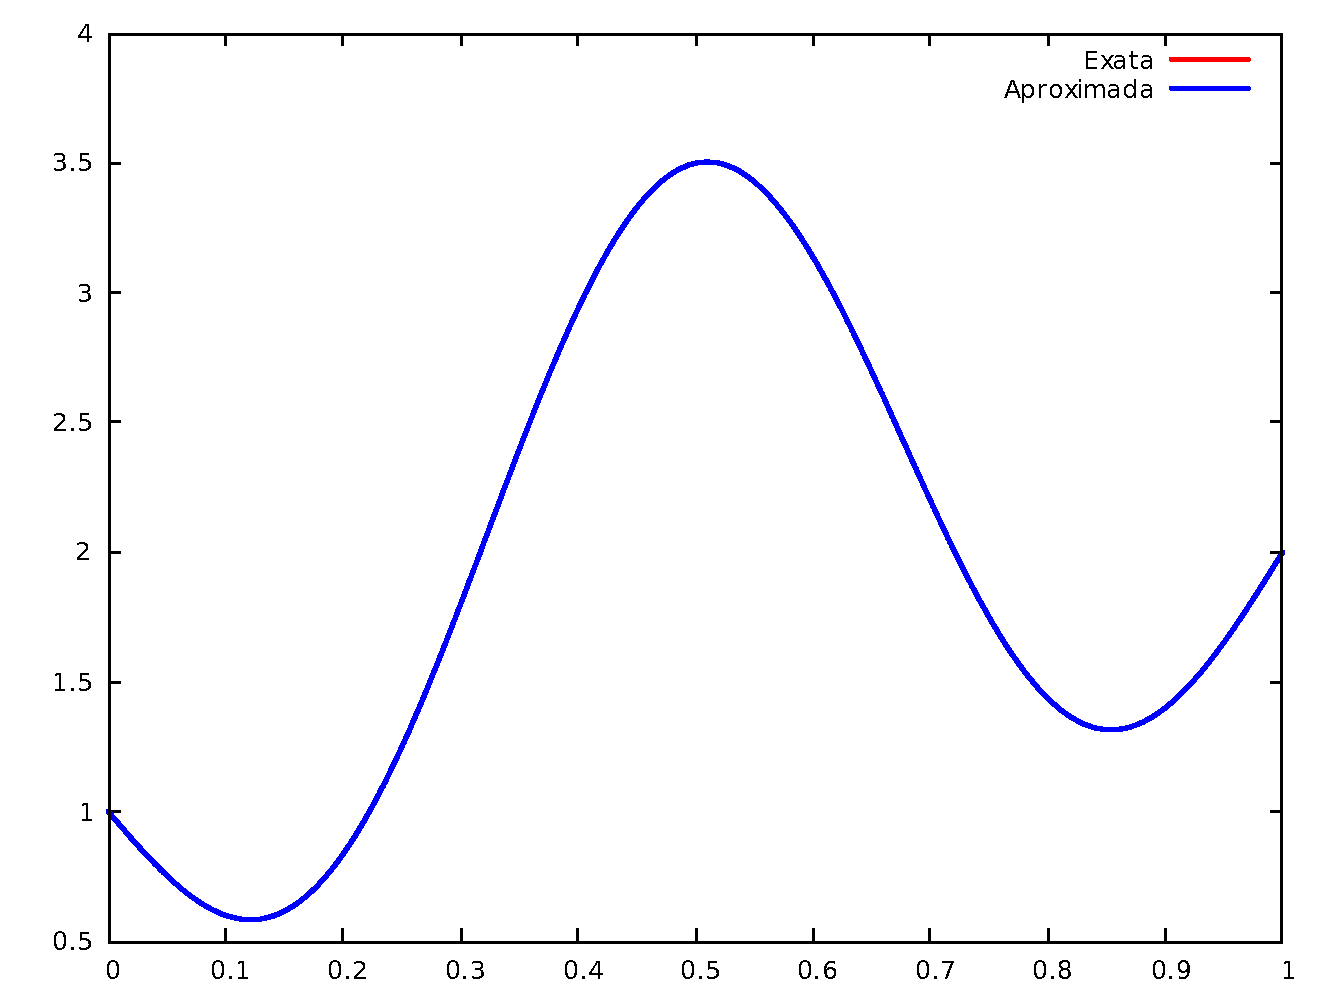
\includegraphics[width=0.48\linewidth]{t3spcub63.pdf}
}
\caption{Resultados com Splines Cúbicos para o Teste 3}
\end{figure}

\begin{table}[H]
\caption{\label{tabla4} Error e Ordem de convergência do Método com Splines Lineares e Splines Cúbicos para o Teste 3.}
\centering
  \begin{tabular}{l|cc|cc}
    \hline
    \hline
    \multirow{2}{*}{\textbf{$n$}} &
      \multicolumn{2}{c}{\textbf{Splines Lineares}} &\multicolumn{2}{c}{\textbf{Splines Cúbicos}} \\
    &\multicolumn{1}{c|}{Error} & \multicolumn{1}{c|}{Ordem} & \multicolumn{1}{c|}{Error} & \multicolumn{1}{c}{Ordem}\\
    \hline
    \hline
	7   & 0.159513968 & - & 4.08572184e-3  & - \\
	15 & 4.60059671e-2 & 3.4672 & 1.81805261e-4 & 22.473\\
	31 & 1.19095291e-2 & 3.8630 & 1.07697491e-5 & 16.881\\
	63 & 3.00329249e-3 & 3.9655 & 6.60525779e-7 & 16.305\\
    \hline
    \hline
  \end{tabular}
\end{table}
\bibliographystyle{apa}
\bibliography{bibliografia}
\end{document}
